% !TeX program = xelatex
% 华为杯 F 题：算力约束下提升大语言模型能力的资源配置建模
\documentclass[zihao=-4,a4paper]{ctexart}

\usepackage{amsmath,amssymb,amsfonts}
\usepackage{bm}
\usepackage{graphicx}
\usepackage{float}
\usepackage{booktabs}
\usepackage{array}
\usepackage{multirow}
\usepackage{caption}
\usepackage{geometry}
\usepackage{enumitem}
\usepackage{xcolor}
\usepackage{listings}
\usepackage{url}

% 按竞赛论文模板设置 A4 纸张和页边距
\geometry{a4paper,left=2.25cm,right=2.25cm,top=3.0cm,bottom=1.85cm}
\graphicspath{{figures/}{../figures/}}

\DeclareCaptionFont{papertext}{\normalfont\songti\zihao{-4}}
\captionsetup{font=papertext,labelfont=papertext,textfont=papertext,labelsep=quad}
\setlength{\parskip}{0.35em}
\setlength{\parindent}{2em}
\linespread{1.0}
\renewcommand{\arraystretch}{1.15}
\AtBeginDocument{\zihao{-4}\songti}

% 格式规范：题目三号黑体，一级标题四号黑体，均居中；其余汉字小四宋体。
% 图内文字按作者要求保留原图样式，不随正文改动。
\ctexset{
  section={format=\normalfont\centering\heiti\zihao{4},beforeskip=1.4ex,afterskip=1.0ex},
  subsection={format=\normalfont\songti\zihao{-4},beforeskip=1.2ex,afterskip=0.8ex},
  subsubsection={format=\normalfont\songti\zihao{-4},beforeskip=1.0ex,afterskip=0.6ex},
  paragraph={format=\normalfont\songti\zihao{-4}},
  subparagraph={format=\normalfont\songti\zihao{-4}}
}

% 附录源代码的排版样式
\renewcommand{\lstlistingname}{代码}
\lstdefinestyle{pythonstyle}{
  language=Python,
  basicstyle=\ttfamily\songti\zihao{-4},
  keywordstyle=\color{blue!70!black},
  commentstyle=\color{green!45!black},
  stringstyle=\color{orange!70!black},
  numbers=left,
  numberstyle=\fontsize{6pt}{7pt}\selectfont\color{gray},
  numbersep=8pt,
  frame=single,
  breaklines=true,
  showstringspaces=false,
  columns=fullflexible,
  tabsize=4,
  captionpos=b
}

\newcommand{\Dt}{D}
\newcommand{\Lctx}{L_{\mathrm{ctx}}}
\newcommand{\Ctrain}{C_{\mathrm{train}}}
\newcommand{\Cattn}{C_{\mathrm{attn}}}
\newcommand{\Deff}{D_{\mathrm{eff}}}



% MH-FLOAT-TUNE 受控浮动调参（防整页空白/一页一图）
\usepackage[section]{placeins}
\usepackage{flafter}
\renewcommand{\topfraction}{0.92}
\renewcommand{\bottomfraction}{0.9}
\renewcommand{\textfraction}{0.06}
\renewcommand{\floatpagefraction}{0.72}
\renewcommand{\dbltopfraction}{0.92}
\renewcommand{\dblfloatpagefraction}{0.72}
\setcounter{topnumber}{3}
\setcounter{bottomnumber}{2}
\setcounter{totalnumber}{4}
\setlength{\textfloatsep}{9pt plus 2pt minus 2pt}
\setlength{\floatsep}{8pt plus 2pt minus 2pt}
\setlength{\intextsep}{8pt plus 2pt minus 2pt}
\usepackage{fancyhdr}

% 页面样式：无页眉，页码位于页脚正中央
\pagestyle{fancy}
\fancyhf{}                  % 清空页眉和页脚
\fancyfoot[C]{\thepage}     % 页脚中央显示页码
\renewcommand{\headrulewidth}{0pt} % 去掉页眉横线
\renewcommand{\footrulewidth}{0pt} % 不显示页脚横线

% 同时覆盖 plain 样式，防止标题页等页面恢复默认样式
\fancypagestyle{plain}{
    \fancyhf{}
    \fancyfoot[C]{\thepage}
    \renewcommand{\headrulewidth}{0pt}
    \renewcommand{\footrulewidth}{0pt}
}
\let\oldcite\cite
\renewcommand{\cite}[1]{\textsuperscript{\oldcite{#1}}}
\usepackage{etoolbox}
% 目录条目采用正文格式；“目录”标题仍按一级标题排版。
\makeatletter
\patchcmd{\l@section}{\bfseries}{\normalfont\songti\zihao{-4}}{}
  {\PackageError{paper}{Cannot set section entry font in contents}{Check the document class.}}
\patchcmd{\l@section}{\addvspace{1.0em \@plus\p@}}{\addvspace{0.3em \@plus\p@}}{}
  {\PackageError{paper}{Cannot compact section spacing in contents}{Check the document class.}}
\makeatother

\begin{document}


% 题目后生成目录，页码连续。
\thispagestyle{fancy}
% 二级目录保持正文小四字号，仅压缩行距，兼顾导航信息和版面利用率。
\begingroup
\setlength{\parskip}{0pt}
\linespread{0.8}\zihao{-4}\selectfont
\setcounter{tocdepth}{2}
\tableofcontents
\endgroup

% 目录后另起一页开始正文
\clearpage

\label{mh:body-start}

\section{问题重述与问题分析}

\subsection{问题背景与任务}
大语言模型的能力主要通过验证集交叉熵损失（全文记为 $L$，单位 nats/token，越低越好）来度量。经典标度律
\begin{equation}
L(N,\Dt)=E+A\,N^{-\alpha}+B\,\Dt^{-\beta},
\label{eq:classic-intro}
\end{equation}
把损失表示为参数规模 $N$ 与训练数据量 $\Dt$ 的幂律叠加，其中 $E$ 为不可约损失，$A,\alpha,B,\beta$ 为待估参数\cite{kaplan2020,hoffmann2022}。然而式~\eqref{eq:classic-intro} 未显式包含数据质量 $Q$ 与领域配比 $\bm p$，也未刻画长上下文对算力的挤占。在总算力预算 $C$ 有限时，如何在 $N,\Dt,Q,\bm p$ 与上下文长度 $\Lctx$ 之间取舍，成为决定模型能力上限的核心问题。本文需要回答四个递进的问题：刻画数据的质量与配比，把它们纳入损失预测，在预算约束下求最优配置，最后把损失翻译为真实基准能力并预测其前沿。

题目提供三组真实数据：一组覆盖七个来源域、含 $22$ 个质量信号的大规模文本样本与两个扩展集；一组来自公开模型训练的标度律轨迹与跨族、文献验证点，其中仅一小组半合成实验带有质量标度；一组开源模型评测榜单、逐任务评测记录、损失—基准桥接样本与模型架构元数据。四问按数据、标度律、预算配置与能力分析组织；实际计算依赖关系在图~\ref{fig:roadmap} 中说明。

\begin{figure}[!htbp]
  \centering
  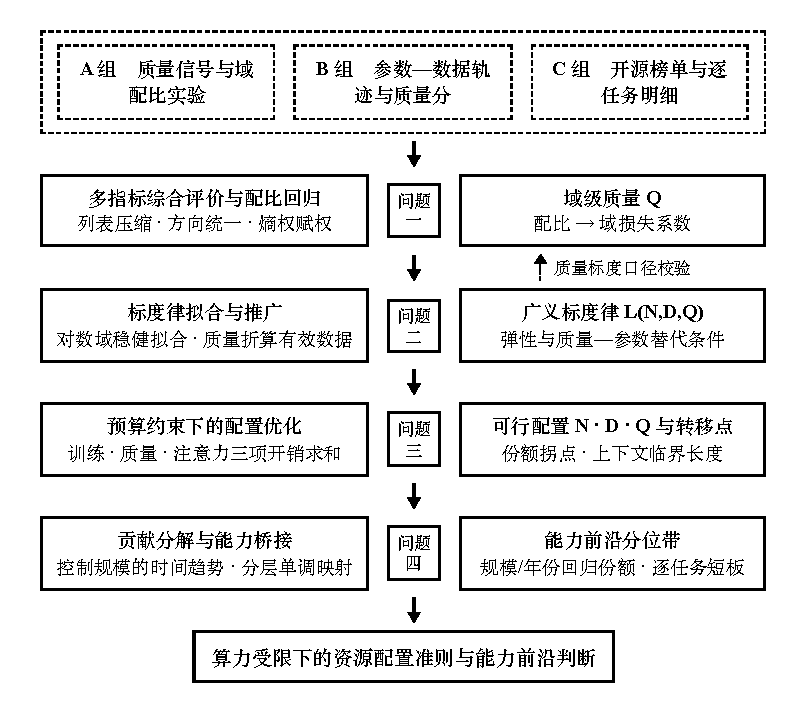
\includegraphics[width=0.88\textwidth,height=0.8\textheight,keepaspectratio]{fig_roadmap.pdf}
  \caption{四问递进的整体技术路线}
  \label{fig:roadmap}
\end{figure}

图~\ref{fig:roadmap} 从左至右给出数据刻画、广义标度律、预算优化与能力预测四个阶段：问题一的域级质量作为问题三基线；配比关系为独立的辅助分析，当前广义律计算固定配比因子为 $1$；标度律参数用于问题三优化目标；问题四的桥接由独立样本拟合；问题四的桥接可探索性地把损失映射到能力，但当前前沿预测直接基于榜单能力值。章节顺序对应问题的分析层次，并不意味着每一项上游量均进入下游数值模型。

\subsection{问题一的分析}
问题一先按字段语义解码二分类与六分类 logits，再用 A1 固定经验百分位、三组平衡权重合成质量；A2/A3 沿用 A1 参照。局部冲突定义为高教育价值且判有广告，降权仅作敏感性对照。配比实验另行拟合分域损失，区分观测留出集与估计值外推表。域级质量进入问题三基线；配比系数未进入广义律或预算优化的数值计算。

\subsection{问题二的分析}
问题二要在经典标度律基础上纳入质量，并讨论配比扩展，是推理密集型任务。首先以真实训练轨迹拟合经典律，并用族外、跨族与文献数据分层验证泛化性；其余轨迹附件登记覆盖情况。广义律的设计是核心：一种自然方式是让高质量数据等效于更多 token，即以有效数据量 $Q^{\theta}\Dt$ 进入数据项，并令 $Q=1$ 时退化为经典形式；半合成实验的质量标度方向与模型假设冲突，质量指数在下游取结构性假定值。弹性与替代条件由对数损失的偏导解析给出，并以有限增量计算检验局部近似的适用范围。本问的广义律与弹性关系是问题三优化目标的来源。

\subsection{问题三的分析}
问题三是“算力约束下的资源配置优化与结构性转移”的混合任务。目标函数取自问题二的广义标度律，约束为基础训练、质量提升与长文本注意力三部分算力之和不超预算。求解上先用 Lagrange/KKT 做解析刻画，预算约束在最优处通常取等号，据此得最优配置关于预算的标度关系；数值上采用预算消元与质量剖面搜索，在三档及连续预算上求候选配置，并以多起点序列二次规划\cite{sqp1995}交叉核验。结构性转移须给出可判定定义，本文以算力份额对预算对数的导数峰值作为数值判据，并检查边界状态。上下文长度依题意为外生参数，须解析给出使注意力开销等于训练开销的临界值并在其可行取值上做敏感性分析。

\subsection{问题四的分析}
问题四是“贡献分解、桥接映射与带不确定性外推”的混合任务。能力提升既来自规模扩张也来自架构、对齐与数据工程等非规模技术进步\cite{gpt3_2020,emergent2022}。以能力对规模变量与时间回归，可作描述性分解；年份项可能混入样本组成和未观测因素，不作因果贡献解释。损失与基准的桥接用按可比性分层的单调映射建立；前沿预测直接用榜单能力值，不传播桥接误差。前沿预测在给定能力趋势系数的情景下外推能力分位带，须显式声明综合能力度量、开源筛选口径与时间轴口径\cite{helm2022,mmlu2020}。本问是全题落点，把前三问的损失语言翻译为现实基准能力。

\subsection{数据证据分层与四问之间的数值接口}
同一附件中的数字承担不同角色，必须先区分“构造评分”“拟合函数”“检验预测”和“设定情景”。例如，A1 的字段可用于定义质量分数，但没有直接给出按该分数筛选后的训练损失；B1 有参数量、训练量和损失，却没有与 A1 同标度的质量标签。将两组数据接入同一个模型，需要显式保留连接假设。本文据此将主要证据分为表~\ref{tab:evidence-levels} 所列的四类。

\begin{table}[!htbp]
\centering\songti\zihao{-4}
\caption{主要附件的证据角色与使用边界}
\label{tab:evidence-levels}
\begin{tabular}{@{}>{\raggedright\arraybackslash}p{2.5cm}>{\raggedright\arraybackslash}p{4.2cm}>{\raggedright\arraybackslash}p{4.2cm}>{\raggedright\arraybackslash}p{3.5cm}@{}}
\toprule
数据类别 & 本文用途 & 可支持的判断 & 不直接支持的判断 \\
\midrule
A1、A2、A3 & 固定参照评分与同名域对照 & 相对评分、冲突发生率 & 评分提高必然降低训练损失 \\
B1、B2、B4、B5 & 经典律拟合与分层验证 & 同族拟合及跨来源误差 & 任意架构上的通用参数 \\
B6--B8 & 质量项的条件预测比较 & 半合成设置内的误差差异 & A1 质量指数的因果估计 \\
估算外推表与趋势情景 & 一致性检查、条件配置和外推 & 假设成立时的数值后果 & 真实未来性能或无条件预测 \\
\bottomrule
\end{tabular}
\end{table}

数值接口按“输入标度一致、单位一致、用途明确”的顺序建立。问题一输出样本评分、域均值和域级中位数；问题三只读取其中的 $Q_0$ 作为质量成本起算点。问题二输出的 B1 经典参数用于资源配置，而半合成经验拟合用于检验质量字段的预测信息，两套参数不拼接。问题四的损失--能力桥接与月度前沿预测也分别计算，前者检验损失和能力之间是否存在可用映射，后者直接描述榜单能力随提交月份的变化。

为使各问结论可追溯，本文对数值结果区分三种来源：从附件直接统计得到的量，例如样本数与域均值；从指定模型估计得到的量，例如经典律系数；从给定参数和情景推导得到的量，例如预算最优配置与两年前沿分位数。第一类也会受抽样和字段定义影响，第二类还会受函数形式影响，第三类则进一步依赖外推假设。后文每次比较均保持数据标度与检验角色一致，不把模型内部的一致性检查当作外部预测验证。

这种分层也决定了问题之间的解释方向。得到较高的相对质量分数，表示在当前参照与权重下更靠近所选指标的有利端；它不能直接转换成提升多少基准分数。预算模型给出的是条件损失最小的配置，仍需在实际训练中确认其损失；即使损失得到验证，能力收益也应在统一基准上再检验。由此形成“数据评分--损失模型--资源配置--能力验证”的完整研究路线，同时明确本题附件已经覆盖与尚未覆盖的环节。


\section{模型假设}
本文只保留会影响可行域、模型结构或结果解释的现实简化，每条附一句合理性说明。

（1）$22$ 个质量字段按类别语义解码并统一方向，用 A1 经验百分位归一化；模型评分、DSIR 和结构信号三组各占 $1/3$。该权重是可检验的建模选择，$Q$ 是相对可用性评分，不是真实质量概率。

（2）领域配比与损失的关系在同一训练尺度内可由配比向量单独预测，参数量与数据量由配比实验固定，分域建模后按目标域加权。数据本按域分列损失，且同配方不同域损失差异显著，支持分域刻画。

（3）质量以“质量增强有效数据量”方式进入广义标度律，令有效数据量为 $Q^{\theta}\Dt$，使 $Q=1$ 时自然退化为经典形式。高质量数据等效于更多 token，物理含义清晰且退化有据。

（4）问题三中配比由前两问固定、仅 $N,\Dt,Q$ 为决策变量，配比联立优化作为扩展。固定配比使规模、数据、质量三者的结构性转移更清晰，且标度律数据无逐域配比字段。

（5）基线质量 $Q_0$ 取问题一七个域级评分的中位数，并在敏感性分析中扰动。题面未给该值；它是当前评分标度下质量成本铰链的起算点，随评分方法变化。

（6）问题四综合能力取六维基准均分，前沿样本要求许可证有明确名称、排除未知及空值，并排除明确关闭权重的记录；时间轴用榜单提交日期，该操作性代理不能核实严格的开源属性。均分口径透明可复现，且题目要求显式声明这些口径。

\section{符号说明}
下表汇总全文跨章节复用、直接进入核心目标或约束的主要符号；一次性下标在首次出现处解释。

\begin{table}[!htbp]
  \centering
  \songti\zihao{-4}
  \begin{tabular}{@{}>{\centering\arraybackslash}p{1.2cm}>{\raggedright\arraybackslash}p{5.3cm}>{\centering\arraybackslash}p{3.9cm}>{\raggedright\arraybackslash}p{4.6cm}@{}}
    \toprule
    符号 & 含义 & 符号 & 含义 \\
    \midrule
    $L$ & 验证集交叉熵损失 (\mbox{nats/token}) & $C$ & 总算力预算 (FLOPs) \\
    $N$ & 模型参数量 ($10^9$) & $\Ctrain$ & 基础训练开销 \\
    $\Dt$ & 训练 token 数 ($10^9$) & $C_Q$ & 质量提升开销 \\
    $Q$ & 综合数据质量评分 $(0,1]$ & $\Cattn$ & 长文本注意力开销 \\
    $Q_0$ & 基线质量 & $\eta$ & 注意力开销系数 $2\times10^{-4}$ \\
    $\bm p$ & $17$ 域配比向量 & $\Lctx$ & 上下文长度 (tokens, 外生) \\
    $E$ & 不可约损失 & $\Lctx^{\mathrm{crit}}$ & 注意力临界上下文 $6/\eta$ \\
    $A,\alpha$ & 参数项系数与指数 & $g(Q)$ & 每 token 质量成本函数 \\
    $B,\beta$ & 数据项系数与指数 & $\varepsilon_X$ & 因素 $X$ 的弹性 \\
    $\theta$ & 质量放大指数 & $s_X$ & 因素 $X$ 的算力份额 \\
    $w_j$ & 质量指标 $j$ 的权重 & $\mathrm{Cap}$ & 综合基准能力 $(0$--$100)$ \\
    \bottomrule
  \end{tabular}
\end{table}

\section{问题一：数据质量评价、冲突识别与配比--损失关系}

本章用 A1 的 $51230$ 条质量信号记录定义样本级质量，用 A2/A3 检验跨集合稳定性；另用 RegMix 配比实验建立配比--损失关系。质量评分与配比回归使用不同附件，后者的系数不进入本章的 $Q$。计算流程见图~\ref{fig:pipeline_q1}。

\begin{figure}[!htbp]
  \centering
  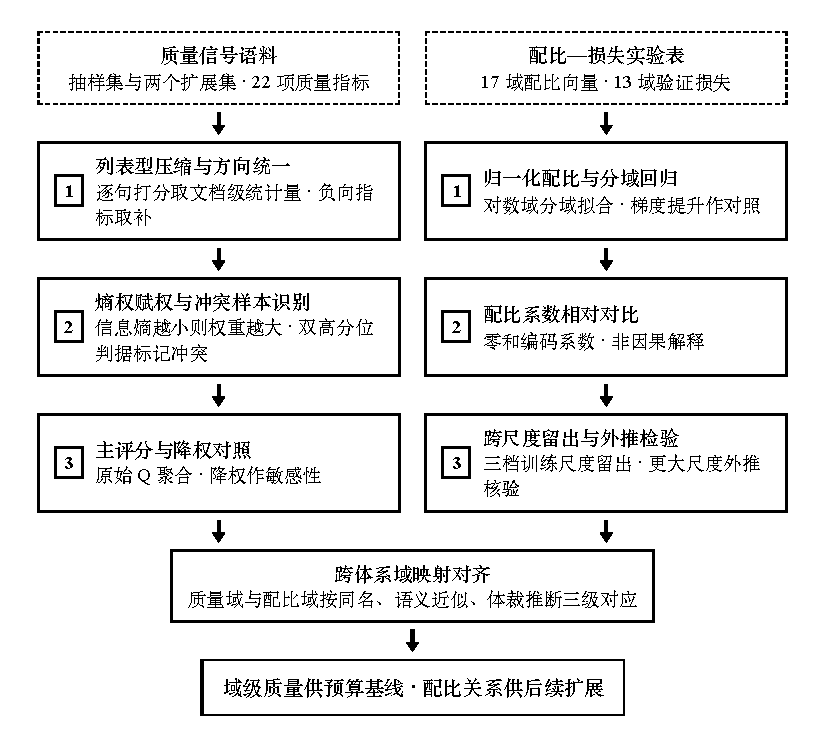
\includegraphics[width=0.96\textwidth,keepaspectratio]{fig_pipeline_q1.pdf}
  \caption{问题一质量评价数据处理流程}
  \label{fig:pipeline_q1}
\end{figure}

\subsection{字段解码、归一化与综合质量}
质量信号覆盖七个来源域、$22$ 个字段。依数据集字段说明\cite{metarater}，\texttt{fluency\_en} 和 \texttt{ad\_en} 是二分类 logits，四个 ModernBERT PRRC 字段是有序六分类 logits；直接对 logits 求均值没有类别含义。二分类取正类 softmax 概率：流畅度取 fluent 类，广告指标取 no-ad 类。六分类取等级 $0,\ldots,5$ 的 softmax 期望并除以 $5$。\texttt{fineweb\_edu} 取单一评分，\texttt{qurater} 的四个评分在字段内等权平均；后者是明确的建模选择。DSIR 与 RPS 标量按原值读入。

缺失值以 A1 同字段中位数填充。词数、句数和平均词长先取 $\log(1+x)$，再截于 A1 的第 $95$ 百分位；重复率、非字母词、大写和数字占比取反向。对方向统一后的字段 $z_{ij}$，固定 A1 经验分布，以中秩百分位评分：
\begin{equation}
r_{ij}=\frac{\#\{z_{kj}<z_{ij}\}+\tfrac12\#\{z_{kj}=z_{ij}\}}{n_{\mathrm{A1}}},\quad k\in\mathrm{A1};\qquad
Q_i=\sum_{j=1}^{22}w_jr_{ij}.
\label{eq:q1-Q}
\end{equation}
扩展集代入同一 A1 参考分布和缺失、截断参数，所得百分位截于 $[0,1]$。模型评分 $8$ 项、DSIR $3$ 项、结构 $11$ 项各占总权重 $1/3$，组内等权，即 $w_j=1/(3n_g)$。域级分数为域内 $Q_i$ 的均值，问题三的 $Q_0$ 取七个域均值的中位数。三组平衡是预先声明的建模选择，所得 $Q$ 不是已校准的真实质量概率。

A1 的 $Q$ 范围为 $0.1459$--$0.8191$，域级中位数 $Q_0=0.48788$。A1 全体均值恰为 $0.500$，是中秩百分位变换的数学性质，不能解释为质量达标率。C4 的域均值最高（$0.55822$），书籍最低（$0.38970$，仅 $171$ 条）。与全局 CRITIC、$22$ 项等权和六分类 argmax 解码相比，七域排序 Kendall 相关依次为 $0.333$、$0.238$、$0.810$。若固定三组各占 $1/3$，仅组内改用 CRITIC，域序不变（Kendall $=1$），域级中位数由 $0.48788$ 变为 $0.48648$；但三组权重各在 $0.2$--$0.5$ 的 $36$ 种网格方案下，域序相关最低为 $0.429$，中位数范围为 $0.455$--$0.511$。主要不确定性在组间权重，不能把单一域排名当作客观质量真值。表~\ref{tab:q1_weights} 给出主权重与 CRITIC 对照，指标结构和相关性见图~\ref{fig:index_hierarchy}、\ref{fig:q1_quality_corr}。

\begin{table}[!htbp]
  \centering
  \caption{三组平衡主权重与 CRITIC 对照}
  \label{tab:q1_weights}
  \songti\zihao{-4}
  \setlength{\tabcolsep}{4pt}
  \begin{tabular}{rlcc@{\hspace{1em}}rlcc}
    \toprule
    \# & 指标 & 主权重 $w_j$ & CRITIC & \# & 指标 & 主权重 $w_j$ & CRITIC \\
    \midrule
    1 & DSIR书籍 & 0.1111 & 0.0506 & 12 & 句末标点 & 0.0303 & 0.0432 \\
    2 & DSIR数学 & 0.1111 & 0.0509 & 13 & 句子数 & 0.0303 & 0.0469 \\
    3 & DSIR维基 & 0.1111 & 0.0507 & 14 & 词数 & 0.0303 & 0.0451 \\
    4 & 流畅度 & 0.0417 & 0.0401 & 15 & 非字母词占比 & 0.0303 & 0.0420 \\
    5 & QuRater & 0.0417 & 0.0390 & 16 & 2gram重复 & 0.0303 & 0.0441 \\
    6 & 无广告概率 & 0.0417 & 0.0478 & 17 & 大写占比 & 0.0303 & 0.0455 \\
    7 & 教育价值 & 0.0417 & 0.0433 & 18 & 唯一词占比 & 0.0303 & 0.0508 \\
    8 & 整洁度 & 0.0417 & 0.0398 & 19 & 数字占比 & 0.0303 & 0.0464 \\
    9 & 推理性 & 0.0417 & 0.0428 & 20 & 平均词长 & 0.0303 & 0.0529 \\
    10 & 专业性 & 0.0417 & 0.0486 & 21 & 3gram重复 & 0.0303 & 0.0445 \\
    11 & 可读性 & 0.0417 & 0.0412 & 22 & unigram熵 & 0.0303 & 0.0440 \\
    \midrule
    \multicolumn{4}{l}{合计 $\sum_j w_j$} & \multicolumn{4}{r}{1.000000} \\
    \bottomrule
  \end{tabular}
\end{table}


表中相同的主权重由“三组各占 $1/3$、组内等权”直接给出，并非熵权计算结果；CRITIC 列是数据驱动的对照，不能据此把主评分称作熵权法。

\begin{figure}[!htbp]
  \centering
  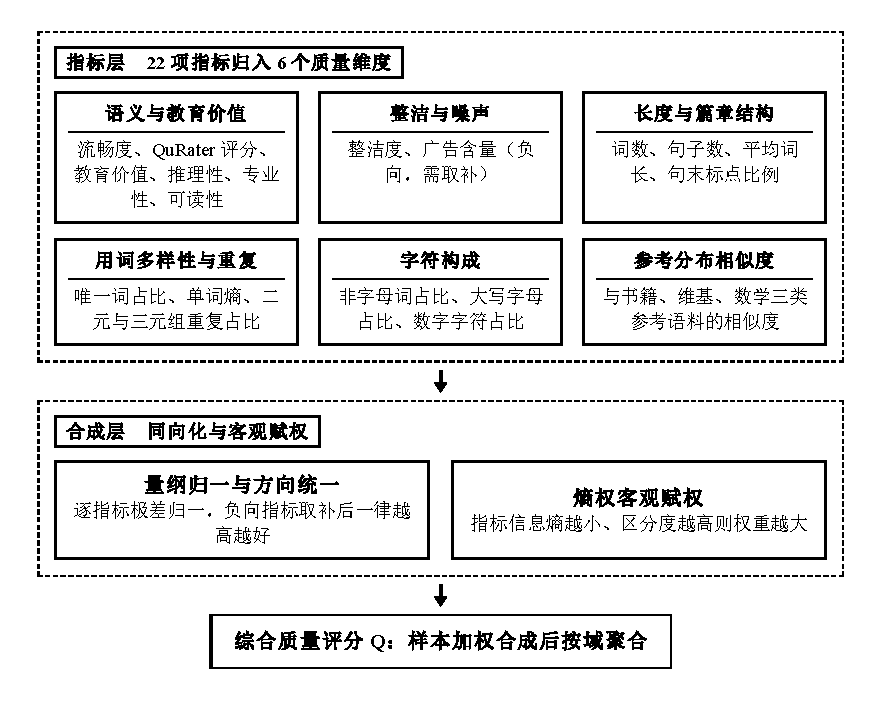
\includegraphics[width=0.96\textwidth,keepaspectratio]{fig_index_hierarchy.pdf}
  \caption{质量指标体系层次结构}
  \label{fig:index_hierarchy}
\end{figure}

\begin{figure}[!htbp]
  \centering
  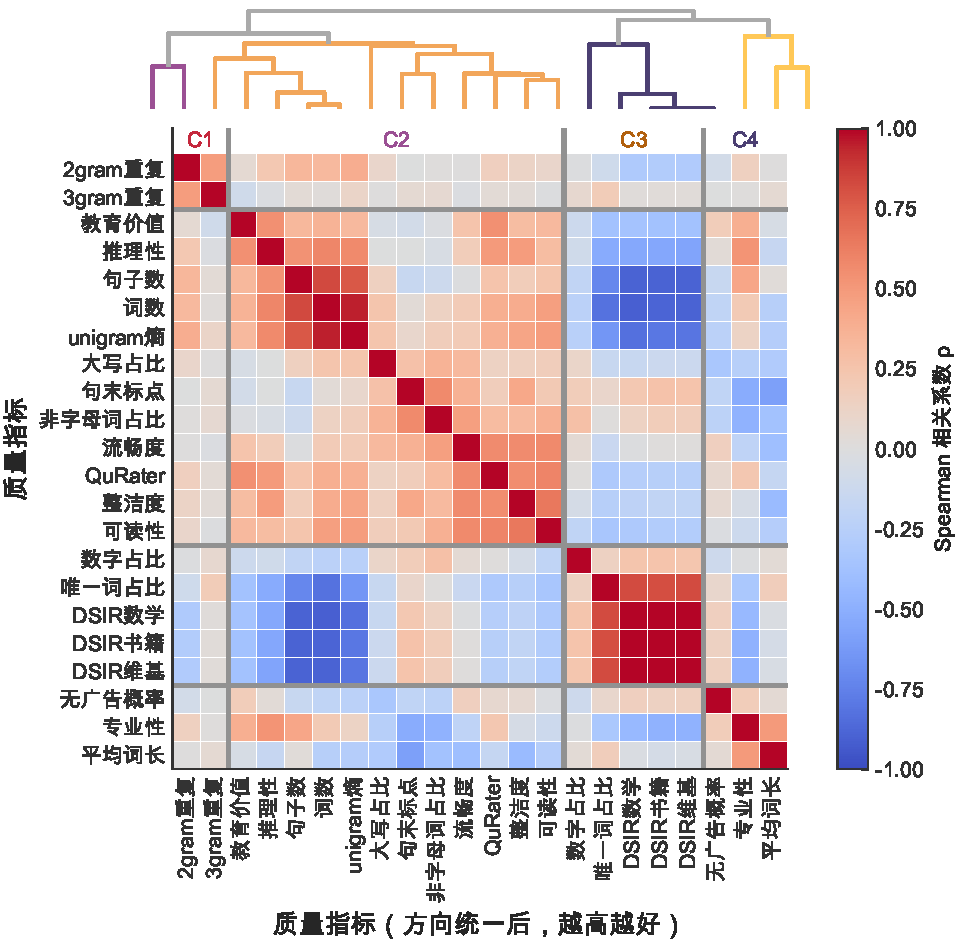
\includegraphics[width=0.92\textwidth,height=0.8\textheight,keepaspectratio]{fig_q1_quality_corr.pdf}
  \caption{语义解码并归一化后质量指标的相关性}
  \label{fig:q1_quality_corr}
\end{figure}

\subsection{质量冲突的判据与对照处理}
冲突定义为同一文档的教育价值位于 A1 前 $20\%$，且二分类模型给出的广告概率超过 $0.5$：
\begin{equation}
{\mathrm{Conflict}}(i)=1\!\left[r_{i,\mathrm{edu}}\geq \tau^{\mathrm{A1}}_{0.8}\;\land\;P_i(\mathrm{has\mbox{-}ad})>0.5\right],
\qquad Q_i^{\rm adj}=\bigl[1-(1-\delta){\mathrm{Conflict}}(i)\bigr]Q_i.
\label{eq:q1-conflict}
\end{equation}
其中 $P(\mathrm{has\mbox{-}ad})=1-P(\mathrm{no\mbox{-}ad})$；$\delta=0.5$ 仅用于对照，主评分与 $Q_0$ 不降权。A2/A3 沿用 A1 的教育价值阈值。

A1 检出 $155/51230$ 条，冲突率 $0.303\%$；C4 为七域最高，$103/10000=1.03\%$。A2 的 arxiv 为 $10/17523=0.057\%$，A3 的 github 为 $24/203752=0.0118\%$。教育价值与广告概率的 A1 Spearman 相关为 $-0.181$，总体负相关与少量局部共现并不矛盾。$\delta\in\{0.3,0.5,0.7,1\}$ 时七域排序不变；降权因子没有下游损失标签校准，故不能声称其提高训练性能。

\begin{figure}[!htbp]
  \centering
  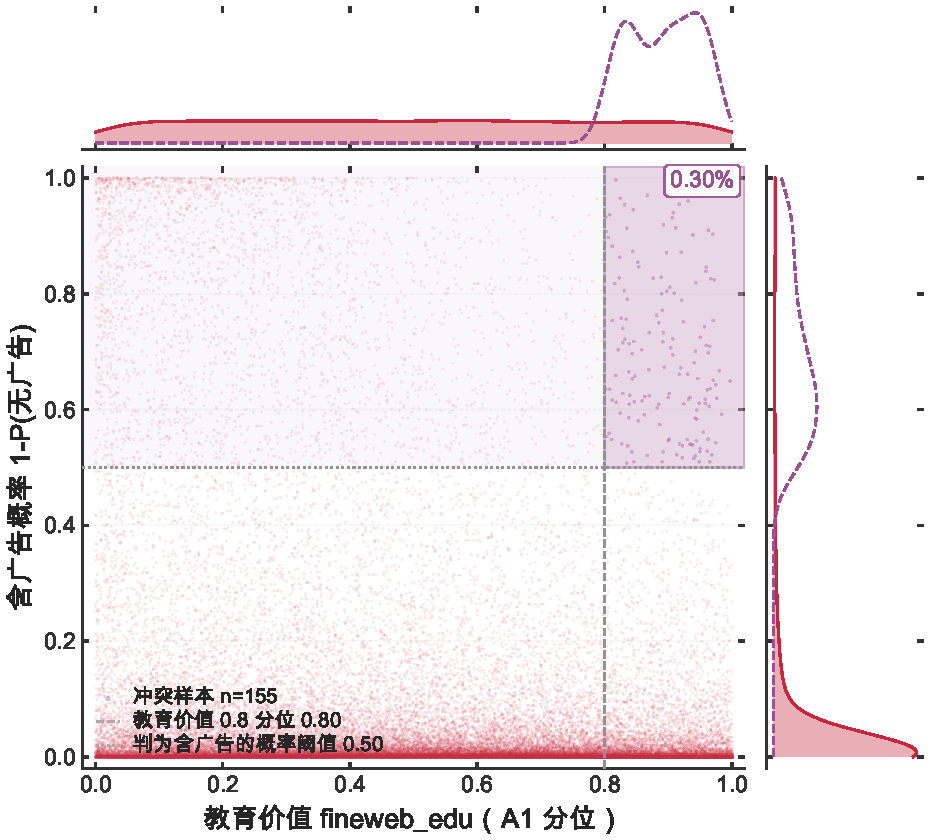
\includegraphics[width=0.92\textwidth,height=0.8\textheight,keepaspectratio]{fig_q1_conflict_scatter.pdf}
  \caption{高教育价值与广告判定的局部共现}
  \label{fig:q1_conflict_scatter}
\end{figure}

\begin{figure}[!htbp]
  \centering
  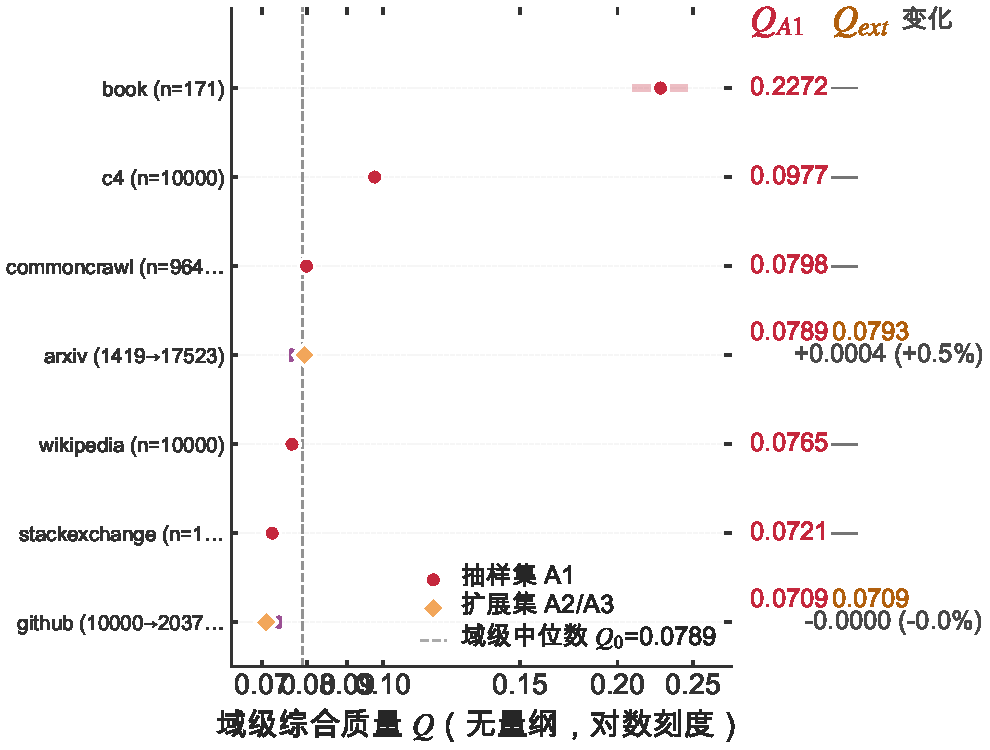
\includegraphics[width=0.9\textwidth,height=0.8\textheight,keepaspectratio]{fig_q1_domain_Q_dumbbell.pdf}
  \caption{A1 抽样域与 A2/A3 扩展域的质量对照}
  \label{fig:q1_domain_Q}
\end{figure}

同一评分参照下，arxiv 的 A1/A2 域均值为 $0.48788/0.48714$，github 的 A1/A3 为 $0.44874/0.44910$。差值分别仅 $-0.00074$ 与 $+0.00036$，说明这两个域的抽样分数较稳定；不能外推到其余五域。表~\ref{tab:q1_domain_Q} 的自助区间只表示 A1 域内抽样波动，不包括评分方案的不确定性。

\begin{table}[!htbp]
  \centering
  \caption{域级综合质量统计}
  \label{tab:q1_domain_Q}
  \songti\zihao{-4}
  \begin{tabular}{lrccrc}
    \toprule
    域 & $n_{A1}$ & $Q_{A1}$ & 95\% 区间 & $n_{ext}$ & $Q_{ext}$ \\
    \midrule
    c4 & 10000 & 0.55822 & [0.55652, 0.55987] & -- & -- \\
    stackexchange & 10000 & 0.50741 & [0.50600, 0.50887] & -- & -- \\
    wikipedia & 10000 & 0.50476 & [0.50335, 0.50627] & -- & -- \\
    arxiv & 1419 & 0.48788 & [0.48656, 0.48907] & 17523 & 0.48714 \\
    commoncrawl & 9640 & 0.48390 & [0.48233, 0.48544] & -- & -- \\
    github & 10000 & 0.44874 & [0.44668, 0.45065] & 203752 & 0.44910 \\
    book & 171 & 0.38970 & [0.38223, 0.39686] & -- & -- \\
    \midrule
    全样本 & 51230 & 0.50000 & -- & -- & -- \\
    \bottomrule
  \end{tabular}
\end{table}


\subsection{配比--损失关系与跨体系域映射}
配比实验给出 $512$ 组 $17$ 维领域配比与对应的 $13$ 域验证损失。对目标域 $k$ 建立对数域线性模型\cite{regmix2024}：
\begin{equation}
\ln \hat L_k(\bm p)=a_k+\sum_{i=1}^{17}b_{ki}p_i,
\qquad p_i\geq 0,\quad \sum_i p_i=1 .
\label{eq:q1-mix}
\end{equation}
单纯形使截距与全部系数不能同时唯一识别；计算中令 $\sum_i b_{ki}=0$ 并相应平移截距，预测不变。平均绝对系数仅描述相对平均配比的模型内对比，不能作因果解释。

$1$m 同尺度留出的平均对数损失 $R^2=0.664$、Spearman $=0.844$；$60$m、$1$B 观测留出集的 $R^2$ 分别为 $-5.387$、$-265.290$，排序相关为 $0.842$、$0.736$。A12--A15 是估计值表，不能当真实留出测试：$10$B/$70$B 的平均 $R^2=-66.863/-81.042$，排序相关 $0.498/0.421$。这些结果表明固定 $1$m 模型不能直接预测大规模绝对损失；跨尺度排序也逐渐变弱。梯度提升模型的 $1$m 五折交叉验证 $R^2=0.977$，只检验同尺度拟合。

\begin{table}[!htbp]
  \centering
  \caption{配比回归分尺度检验；末两行是附件估计值}
  \label{tab:q1-mixture-holdout}
  \songti\zihao{-4}
  \begin{tabular}{lrrr}
    \toprule
    尺度 & 配比数 & 平均 $\ln L$ 的 $R^2$ & 平均 Spearman \\
    \midrule
    $1$m & 256 & $0.664$ & $0.844$ \\
    $60$m & 256 & $-5.387$ & $0.842$ \\
    $1$B & 64 & $-265.290$ & $0.736$ \\
    $10$B（估计） & 63 & $-66.863$ & $0.498$ \\
    $70$B（估计） & 63 & $-81.042$ & $0.421$ \\
    \bottomrule
  \end{tabular}
\end{table}

\begin{figure}[!htbp]
  \centering
  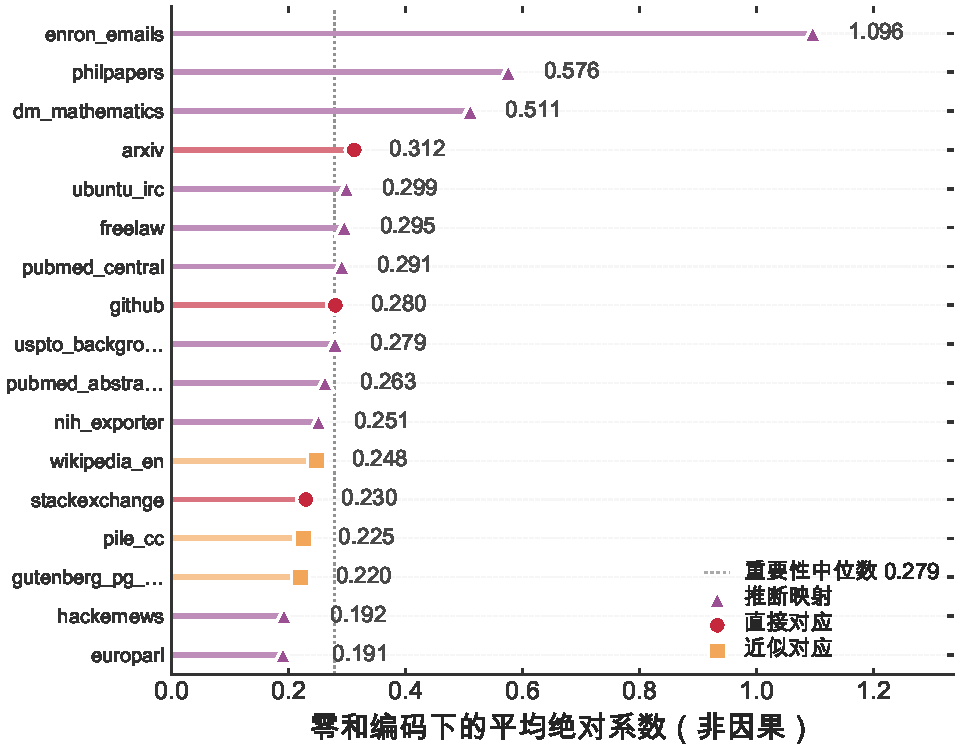
\includegraphics[width=0.9\textwidth,height=0.8\textheight,keepaspectratio]{fig_q1_mixture_importance.pdf}
  \caption{零和编码下配比系数的相对对比强度}
  \label{fig:q1_mixture_imp}
\end{figure}

质量域与配比的 $17$ 个域并不一一对应。依据附件映射指南，三个域可同名对应、三个域语义近似对应，其余是推断映射；无质量域的配比列仍保留在式~\eqref{eq:q1-mix} 中。推断映射只为后续解释提供参考，不产生新的观测质量值，也未进入问题三数值求解。

\subsection{小结}
问题一给出七域质量中位数 $Q_0=0.48788$ 与明确判据下的 A1 冲突率 $0.303\%$。二者均依赖所选评分标度和阈值。配比模型的跨尺度绝对损失预测显著失准，暂不用于预算配置。

\section{问题二：经典标度律拟合与含质量的广义标度律}

本章先在真实训练轨迹上拟合经典标度律，再构造含质量的有效数据量扩展，并解析弹性与质量对规模的替代条件。配比影响在本章保留为待识别扩展，数值计算固定其因子为 $1$；问题三使用这里的损失参数，问题四的桥接由另一组损失--基准样本独立拟合。

\subsection{经典标度律的对数域稳健拟合}
采用题目给定的经典形式式~\eqref{eq:classic-intro}。以 $1176$ 行真实 Pythia 训练日志\cite{pythia2023}为主拟合集（参数量 $0.07$--$12$B、数据量至 $300$B）。由于损失跨越约 $2$ 到 $4.7$ 的量级，直接在原始尺度最小二乘会被大损失点主导，故在对数域用 Huber 损失做加权非线性最小二乘，兼顾同方差化与对离群轨迹点的稳健性：
\begin{equation}
\min_{E,A,\alpha,B,\beta}\ \sum_{m=1}^{M}\rho_\kappa\!\Bigl(\ln L_m-\ln\bigl(E+A N_m^{-\alpha}+B \Dt_m^{-\beta}\bigr)\Bigr),\quad
\rho_\kappa(u)=\begin{cases}\tfrac12 u^2, & |u|\le\kappa,\\[2pt]\kappa\bigl(|u|-\tfrac12\kappa\bigr), & |u|>\kappa.\end{cases}
\label{eq:q2-huber}
\end{equation}
求解用信赖域反射的非线性最小二乘并启用 Huber 稳健损失，以 $\alpha,\beta\in[0.05,0.5]$ 的网格初值多起点启动，避免落入局部解。

\textbf{结果与分层验证。}拟合得 $E=1.690$、$A=0.354$、$\alpha=0.340$、$B=1.240$、$\beta=0.280$，决定系数 $R^2$ 接近 $1$，残差均值约 $-5\times10^{-8}$。两个指数落在文献常见区间 $(0,1)$ 内，且方向正确——增大参数量或数据量都使损失下降\cite{kaplan2020,hoffmann2022}。为考察泛化，在四组独立数据上分层验证：族外半合成日志、插值轨迹、$12$ 族收敛点与文献点，其中跨族基线决定系数 $0.60$、文献点 $0.73$，均方根误差随可比性下降而增大，符合预期。百亿参数以上的估算点仅用于外推讨论，不作为观测。图~\ref{fig:q2_scaling_fit} 给出拟合优度与残差。

\begin{figure}[H]
  \centering
  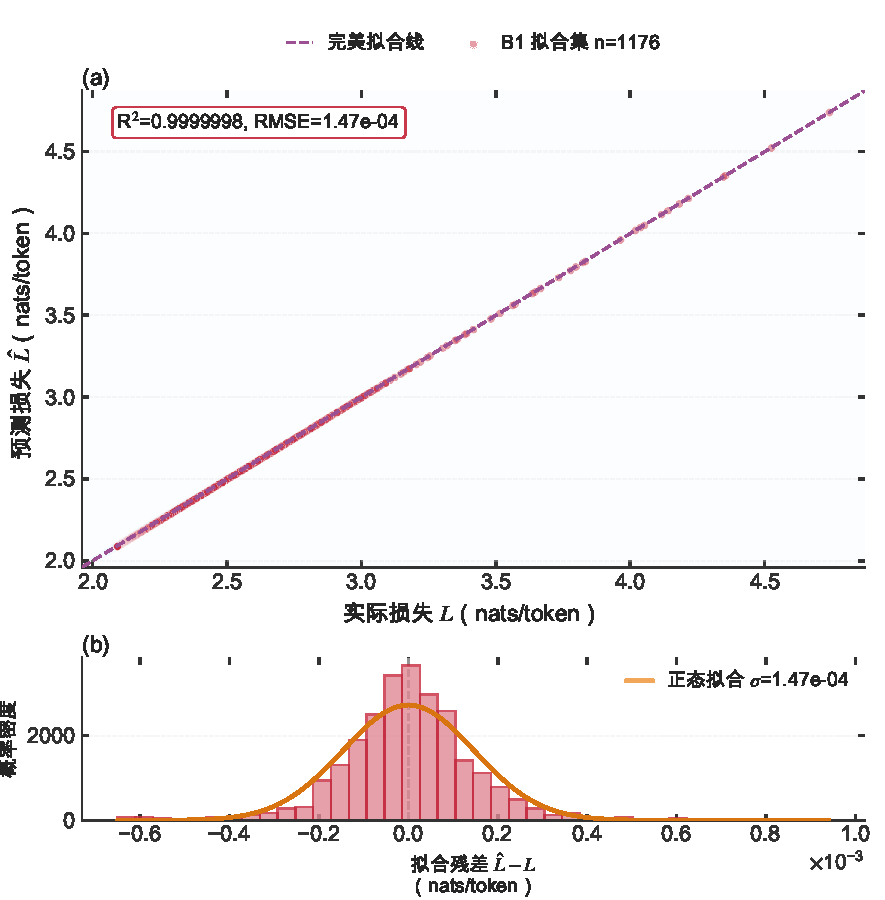
\includegraphics[width=0.8\textwidth,height=0.8\textheight,keepaspectratio]{fig_q2_scaling_fit.pdf}
  \caption{经典标度律拟合优度与残差}
  \label{fig:q2_scaling_fit}
\end{figure}

预测--实际散点几乎落在对角线上，拟合残差 $\hat L-L$ 在零线附近无系统弯曲（残差标准差约 $1.5\times10^{-4}$ nats/token，量级远小于 $L$ 本身），说明经典幂律在真实轨迹上的拟合已相当充分，可作为广义律的可靠基底（图~\ref{fig:q2_scaling_fit}，右图横轴为残差 $\hat L-L$，单位 nats/token）。

\subsection{含质量的广义标度律设计}
经典律未含质量。本文让高质量数据等效于更多 token，即以有效数据量 $\Deff=Q^{\theta}\Dt$（$\theta>0$）进入数据项：
\begin{equation}
\boxed{\,L(N,\Dt,Q)=E+A\,N^{-\alpha}+B\,\bigl(Q^{\theta}\Dt\bigr)^{-\beta}\,}.
\label{eq:q2-gen}
\end{equation}
当 $Q=1$ 时 $Q^{\theta}=1$、$\Deff=\Dt$，式~\eqref{eq:q2-gen} 在代数上退化为经典式~\eqref{eq:classic-intro}。问题一的 $Q$ 是 A1 相对百分位的加权评分，$1$ 是模型边界，没有经验样本被证明达到“完美质量”。评分还含文档长度信号；把 $Q^{\theta}\Dt$ 解作有效 token 数是建模假设，其独立质量效应尚缺真实质量--损失联合观测验证。配比调节项 $\phi(\bm p)$ 可作为扩展，但当前拟合和问题三计算均固定 $\phi=1$。

\textbf{质量放大指数的不可识别性与结构性取值。}原则上质量放大指数 $\theta$ 应由带质量标度的半合成实验估计，这也是全部数据中唯一含质量标度的来源。但实测发现该实验的质量标度与验证损失呈\emph{正相关}（Spearman 约 $+0.446$，组内更高），即“质量标度越高损失越高”，与“高质量有益”的方向相反，且在极低质量标度处损失甚至低于经典不可约损失。这说明该实验的质量标度并非问题一的部署质量口径，而是重标定损失区间的\emph{实验设定量}（难度或多样性指标），$\theta$ 无法从该数据中识别。为避免把无根据的经验值伪装成估计结果，本文明确将 $\theta$ 定位为\textbf{结构性假定参数}而非估计量：取 $\theta=0.5$ 只是位于“质量无效”（$\theta=0$）与“质量和数据等弹性”（$\theta=1$）之间的示例设定，不是数据估计值，也没有特别的统计最优性。另以 $\{0.2,0.5,0.8\}$ 做情景敏感性分析；只在这些设定下讨论相应结果。据此所有依赖 $\theta$ 的下游结论（问题三最优配置）均在“$\theta=0.5$ 假定下成立”的限定下解读，并在 $\{0.2,0.5,0.8\}$ 上给出敏感性区间。需说明含质量广义律在留出集上的均方根误差 $0.688$ 低于同参经典基线的 $0.971$，反映的是引入质量维度后模型自由度与拟合灵活性的提升，而非对 $\theta$ 绝对值的验证。表~\ref{tab:q2_scaling} 汇总两律的参数与拟合优度。

\begin{table}[H]
  \centering
  \caption{标度律参数与拟合优度}
  \label{tab:q2_scaling}
  \small
  \begin{tabular}{lrr}
    \toprule
    项 & 经典律 $L(N,D)$ & 广义律 $L(N,D,Q)$ \\
    \midrule
    \multicolumn{3}{l}{\textit{参数}} \\
    \quad $E$ & 1.6898 & 0.2163 \\
    \quad $A$ & 0.3540 & 0.5311 \\
    \quad $\alpha$ & 0.3400 & 0.3090 \\
    \quad $B$ & 1.2403 & 2.9534 \\
    \quad $\beta$ & 0.2799 & 0.1228 \\
    \quad $\theta$ (经验) & -- & -10.000 \\
    \quad $\theta$ (下游取用) & -- & 0.50 \\
    \midrule
    \multicolumn{3}{l}{\textit{拟合}} \\
    \quad 样本量 $n$ & 1176 & 2012 \\
    \quad $R^2$ & 0.9999998 & 0.3389 \\
    \quad 残差标准差 & 1.466e-04 & -- \\
    \quad AIC & -31.6 & -1842.7 \\
    \quad BIC & -2.5 & -1807.8 \\
    \midrule
    \multicolumn{3}{l}{\textit{留出/外部集 RMSE}} \\
    \quad B6 留出 ($n$=502) & 0.9713 & 0.6879 \\
    \quad published ($n$=44) & 0.1976 & -- \\
    \quad baseline ($n$=57) & 0.2927 & -- \\
    \quad cerebras ($n$=1029) & 1.2431 & -- \\
    \midrule
    \multicolumn{3}{l}{\textit{参考点弹性}} \\
    \quad $\varepsilon_N$ & -- & -0.0657 \\
    \quad $\varepsilon_D$ & -- & -0.0860 \\
    \quad $\varepsilon_Q$ & -- & -0.0430 \\
    \quad $dN/dQ|_L$ & -- & -1.3097 \\
    \bottomrule
  \end{tabular}
\end{table}


经典律与广义律的参数对比见表~\ref{tab:q2_scaling}：经典律以近乎完美的 $R^2$ 拟合真实轨迹；广义律行中的经验质量指数因上述设定量口径问题落在边界（不可识别），故表中明确标注为“不可识别，下游取用结构性假定值 $\theta=0.5$”，这一分列正是对数据与假设冲突的诚实呈现，而非把数据改写以迎合假设。$Q=1$ 退化的相对误差为 $0$，满足等价性要求。广义律的损失曲面见图~\ref{fig:q2_gen_surface}。

\begin{figure}[H]
  \centering
  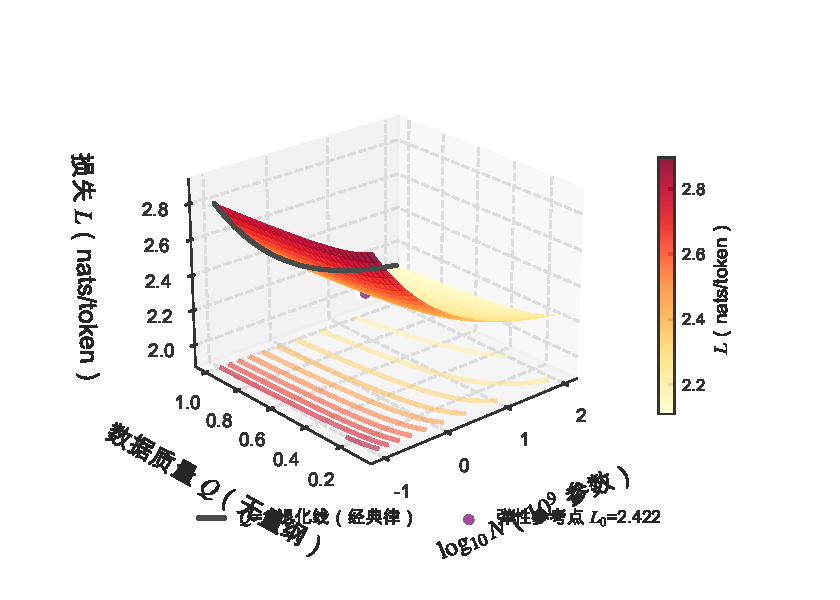
\includegraphics[width=0.96\textwidth,height=0.8\textheight,keepaspectratio]{fig_q2_generalized_surface.pdf}
  \caption{广义标度律损失曲面}
  \label{fig:q2_gen_surface}
\end{figure}

固定数据量后，损失随参数量与质量的联合变化面沿任一方向增大均单调下降，质量方向的下降经 $Q^{\theta}$ 放大数据项体现，直观展示了质量与规模对损失的协同作用（图~\ref{fig:q2_gen_surface}，含 $Q=1$ 退化对照线）。

\subsection{弹性、边际效用与质量--规模替代}
定义因素 $X$ 的弹性 $\varepsilon_X=\partial\ln L/\partial\ln X$。对广义律式~\eqref{eq:q2-gen} 求偏导得
\begin{equation}
\frac{\partial L}{\partial N}=-\alpha A N^{-\alpha-1},\quad
\frac{\partial L}{\partial \Dt}=-\beta B Q^{-\theta\beta}\Dt^{-\beta-1},\quad
\frac{\partial L}{\partial Q}=-\theta\beta B Q^{-\theta\beta-1}\Dt^{-\beta},
\label{eq:q2-partials}
\end{equation}
从而
\begin{equation}
\varepsilon_N=\frac{-\alpha A N^{-\alpha}}{L},\qquad
\varepsilon_D=\frac{-\beta B (Q^{\theta}\Dt)^{-\beta}}{L},\qquad
\varepsilon_Q=\theta\,\varepsilon_D .
\label{eq:q2-elastic}
\end{equation}
式~\eqref{eq:q2-elastic} 表明质量弹性是数据弹性的 $\theta$ 倍：质量通过放大有效数据发挥作用，其边际效用与数据同向而幅度可调。沿等损失面 $\mathrm dL=0$，质量与规模的替代率为
\begin{equation}
\left.\frac{\mathrm dN}{\mathrm dQ}\right|_{L}=-\frac{\partial L/\partial Q}{\partial L/\partial N}
=-\frac{\theta\beta B\,Q^{-\theta\beta-1}\Dt^{-\beta}}{\alpha A\,N^{-\alpha-1}} .
\label{eq:q2-subst}
\end{equation}

\textbf{结果。}在参考点（参数量 $1$、数据量 $100$、质量 $0.5$）代入拟合参数，得 $\varepsilon_N=-0.066$、$\varepsilon_D=-0.086$、$\varepsilon_Q=-0.043$，三者均为负、方向正确，且满足 $\varepsilon_Q=\theta\varepsilon_D$。替代率 $\mathrm dN/\mathrm dQ|_L=-1.31$，即在该参考点把质量提升 $0.1$ 约等价于减少 $0.13\times10^9$ 参数而保持损失不变——质量确可在一定范围内替代规模。需强调该数值强依赖假定的质量指数，故其量级仅在参考点邻域可信，正负号由所设正质量指数的模型形式决定，不构成独立经验验证。图~\ref{fig:q2_elasticity} 与图~\ref{fig:q2_substitution} 分别展示弹性对照与替代关系。

\begin{figure}[H]
  \centering
  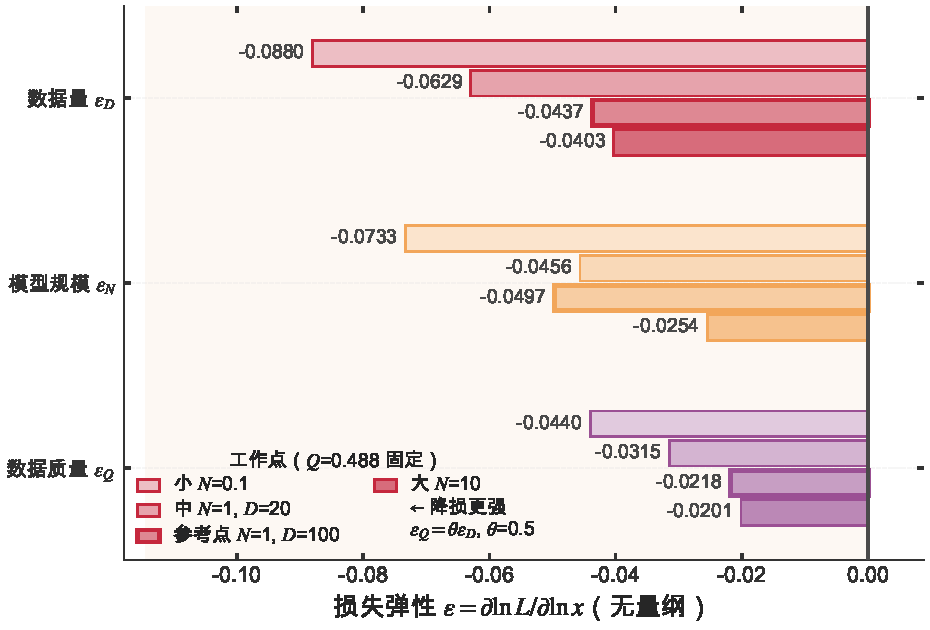
\includegraphics[width=0.9\textwidth,height=0.8\textheight,keepaspectratio]{fig_q2_elasticity_diverging.pdf}
  \caption{各因素损失弹性对照}
  \label{fig:q2_elasticity}
\end{figure}

三个弹性中数据弹性绝对值最大、参数次之、质量最小，说明在该参考点数据量的边际效用最高；三者同为负值再次确认增大任一因素都降低损失（图~\ref{fig:q2_elasticity}）。

\begin{figure}[H]
  \centering
  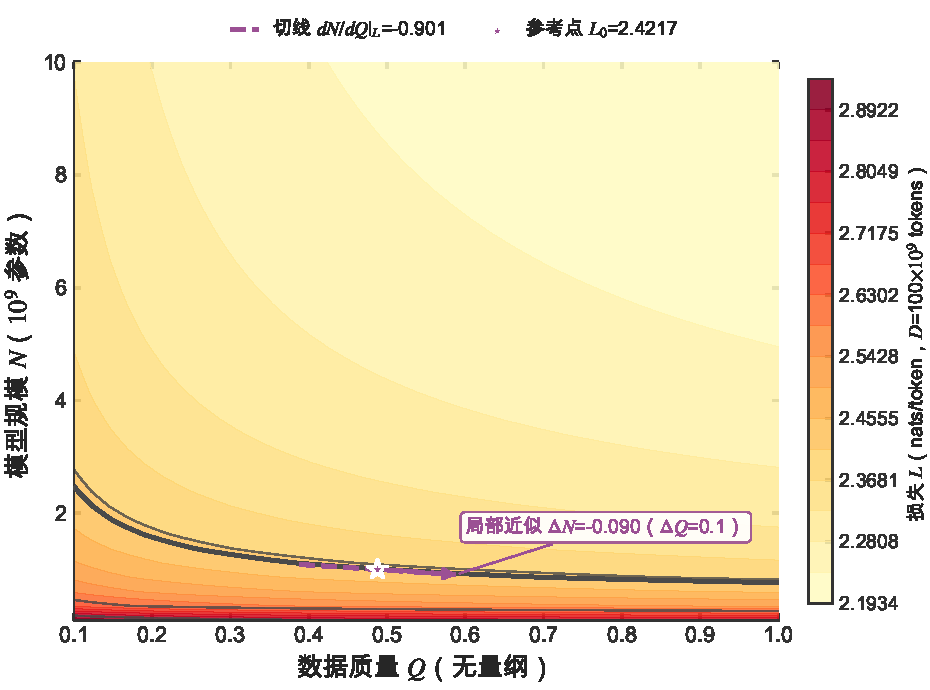
\includegraphics[width=0.9\textwidth,height=0.8\textheight,keepaspectratio]{fig_q2_substitution_contour.pdf}
  \caption{等损失线与质量--规模替代}
  \label{fig:q2_substitution}
\end{figure}

等损失曲线在低质量区更陡（图~\ref{fig:q2_substitution}），其斜率即式~\eqref{eq:q2-subst} 给出的质量--规模即时替代率，表明质量越低时提升质量替代规模的效率越高。这一分析为问题三在预算约束下权衡质量投入与规模扩张提供了边际依据。

\section{问题三：算力约束下的资源配置优化与结构性转移}

本章在总算力预算有限时，求使损失最小的参数量、数据量与质量配置，并分析预算跨量级时最优策略是否发生质变。目标函数取自问题二的广义标度律，约束为三部分算力之和不超预算。

\subsection{优化模型}
决策变量为参数量 $N>0$、数据量 $\Dt>0$ 与质量 $Q\in(0,1]$。$N,\Dt$ 分别以十亿参数、十亿 token 为单位；记 $U=10^9$，则物理计数为 $UN,U\Dt$。上下文长度 $\Lctx$ 为外生参数，配比在当前数值模型中固定。目标与 FLOPs 约束为
\begin{align}
\min_{N,\Dt,Q}\ & L(N,\Dt,Q)=E+A\,N^{-\alpha}+B\,\bigl(Q^{\theta}\Dt\bigr)^{-\beta},
\label{eq:q3-obj}\\
\text{s.t.}\ & \underbrace{6U^2N\Dt}_{\Ctrain}
+\underbrace{U\Dt\,[g(Q)-g(Q_0)]_+}_{C_Q}
+\underbrace{\eta U^2N\Dt\Lctx}_{\Cattn}\ \le\ C,
\label{eq:q3-budget}\\
& 0<Q\le 1,\qquad N>0,\ \Dt>0,
\label{eq:q3-dom}
\end{align}
其中基础训练开销取 Chinchilla 系数 $6$（每参数每 token 约 $6$ FLOPs，仅在标准 dense transformer 下成立；MoE 等稀疏架构需按激活比例折算，本文优化的模型族均按 dense 处理）。注意力开销是工程一阶近似，$\eta=2\times10^{-4}$；它刻画长上下文挤占预算的趋势，不作逐架构的精确 FLOPs 计数。$g(Q)$ 为每个物理 token 的质量成本（FLOPs/token），取指数、幂、对数三型之一；$[\cdot]_+$ 表示仅当质量超过基线 $Q_0$ 时才计增量成本。$Q_0=0.079$ 取自问题一域级质量中位数。显式写出 $U$ 可避免把“十亿”为单位的标度律变量直接代入物理 FLOPs 公式。

\subsection{KKT 解析刻画}
预算约束在最优处通常取等号，因为增大任一因素都降损失、必用尽预算。在 $Q>Q_0$ 的活跃段构造 Lagrange 函数
\begin{equation}
\mathcal L=E+A N^{-\alpha}+B(Q^{\theta}\Dt)^{-\beta}
+\mu\bigl(U^2N\Dt(6+\eta\Lctx)+U\Dt[g(Q)-g(Q_0)]-C\bigr),
\label{eq:q3-lagr}
\end{equation}
其一阶条件为
\begin{align}
\partial_N\mathcal L&=-\alpha A N^{-\alpha-1}+\mu U^2\Dt(6+\eta\Lctx)=0,
\label{eq:q3-kkt-n}\\
\partial_D\mathcal L&=-\beta B Q^{-\theta\beta}\Dt^{-\beta-1}
+\mu\bigl(U^2N(6+\eta\Lctx)+U[g(Q)-g(Q_0)]\bigr)=0,
\label{eq:q3-kkt-d}\\
\partial_Q\mathcal L&=-\theta\beta B Q^{-\theta\beta-1}\Dt^{-\beta}
+\mu U\Dt\,g'(Q)=0 .
\label{eq:q3-kkt-q}
\end{align}
由式~\eqref{eq:q3-kkt-n}--\eqref{eq:q3-kkt-d} 可消去乘子 $\mu$，得到参数量与数据量的边际平衡关系\cite{hoffmann2022}。质量条件须分段理解：$Q<Q_0$ 时提高质量不增加 $C_Q$ 却降低损失，故候选最优解不会停在该段；在 $Q=Q_0$ 处比较铰链两侧的单边导数，在 $Q_0<Q<1$ 的内点使用式~\eqref{eq:q3-kkt-q} 的边际收益等于边际成本条件，在 $Q=1$ 时检查上界条件。以上均为局部必要条件，不能单独证明全局最优。

\subsection{数值求解}
KKT 给出候选解的局部条件；数值上用序列二次规划配合多起点搜索\cite{sqp1995}。为避免变量尺度悬殊，对参数量与数据量取对数尺度 $(\ln N,\ln\Dt,Q)$，预算约束以非线性约束形式送入求解器；每档预算取不少于 $20$ 个初值，报告其中损失最低的可行解；多起点搜索不能证明全局最优。三档预算 $C\in\{10^{19},10^{22},10^{24}\}$，并在预算对数区间连续扫描以刻画转移；三型质量成本分别求解以比较其对最优解的影响。表~\ref{tab:q3_allocation} 汇总结果。

\textbf{可复现求解步骤。}
\begin{enumerate}[leftmargin=2em,itemsep=0pt,topsep=0.2em]
  \item 固定预算 $C$、成本函数 $g$ 与上下文长度；以式~\eqref{eq:q3-budget} 构造归一化可行余量 $(C-C_{\mathrm{tot}})/C\ge0$。
  \item 在 $(\ln N,\ln\Dt,Q)$ 空间取一个近似规模--数据平衡初值和其余随机初值，随机种子固定为 $42$；数值边界取 $N\in[10^{-3},10^5]$、$\Dt\in[10^{-2},10^6]$、$Q\in[10^{-3},1]$。三档主预算各用 $20$ 个初值，连续预算扫描用 $12$ 个。
  \item 对每个初值运行 SLSQP（最多 $500$ 次迭代，目标容差 $10^{-12}$）；只保留重算后满足 $C_{\mathrm{tot}}\le C(1+10^{-6})$ 的候选，按损失选最低者。该可行性筛选不等于全局最优证书。
\end{enumerate}
结构转移计算在 $\log_{10}C\in[18,25]$ 的 $36$ 个网格点上重复搜索，再对质量算力份额作数值差分；网格峰值应视作候选位置而非精确物理阈值。
以指数型质量成本和 $C=10^{22}$ FLOPs 为例，候选配置为约 $5.52$B 参数、$258.6$B token、$Q=0.968$。代回物理成本式，基础训练、质量与注意力开销分别约占预算的 $0.856$、$0.086$、$0.058$，三项之和约为 $1$。这一回代检验能发现单位错误或越预算解，但不能检验损失模型在该配置处的外推精度。

\begin{table}[H]
  \centering
  \caption{三档预算下的最优算力配置}
  \label{tab:q3_allocation}
  \small
  \resizebox{\textwidth}{!}{%
  \begin{tabular}{llrrrrrrr}
    \toprule
    $C$ (FLOPs) & $g(Q)$ & $N^*$ & $D^*$ & $Q^*$ & $L^*$ & $s_{train}$ & $s_Q$ & $s_{attn}$ \\
    \midrule
    $10^{19}$ & 指数型 & 0.193 & 7.9 & 0.5057 & 3.0729 & 0.9205 & 0.0167 & 0.0628 \\
     & 幂型 & 0.188 & 8.3 & 0.4879 & 3.0731 & 0.9361 & 0.0000 & 0.0639 \\
     & 对数型 & 0.188 & 8.3 & 0.4879 & 3.0731 & 0.9361 & 0.0000 & 0.0639 \\
    & Chinchilla 基线 & 1.249 & 1.2 & 0.4879 & 3.3066 & 0.9361 & 0.0000 & 0.0639 \\
    \midrule
    $10^{22}$ & 指数型 & 5.483 & 261.4 & 0.9665 & 2.1507 & 0.8600 & 0.0813 & 0.0587 \\
     & 幂型 & 5.758 & 240.3 & 1.0000 & 2.1525 & 0.8300 & 0.1133 & 0.0567 \\
     & 对数型 & 5.225 & 287.8 & 1.0000 & 2.1458 & 0.9023 & 0.0361 & 0.0616 \\
    & Chinchilla 基线 & 39.499 & 39.5 & 0.4879 & 2.2813 & 0.9361 & 0.0000 & 0.0639 \\
    \midrule
    $10^{24}$ & 指数型 & 40.740 & 3773.9 & 1.0000 & 1.9139 & 0.9225 & 0.0145 & 0.0630 \\
     & 幂型 & 40.893 & 3747.8 & 1.0000 & 1.9140 & 0.9195 & 0.0177 & 0.0628 \\
     & 对数型 & 40.280 & 3854.6 & 1.0000 & 1.9136 & 0.9316 & 0.0048 & 0.0636 \\
    & Chinchilla 基线 & 394.989 & 395.0 & 0.4879 & 1.9935 & 0.9361 & 0.0000 & 0.0639 \\
    \bottomrule
  \end{tabular}
  }
\end{table}


预算增大时最优损失单调下降（指数型下从 $3.098$ 经 $2.151$ 降至 $1.914$），逐步趋近不可约损失 $1.69$，参数量与数据量单调增，预算利用率约 $100\%$（约束活跃）；相对质量固定为基线、规模等分的 Chinchilla 基线方案，最优配置的损失改善约 $0.15$ 到 $0.58$（表~\ref{tab:q3_allocation}）。三型质量成本的最优解在中高预算趋于一致，仅在低预算档因质量成本经济性不同而分化：对数型使高质量相对可得，故低预算即把质量推到边界；指数型使高质量昂贵，故低预算下质量停在内点。三档预算的算力份额构成见图~\ref{fig:q3_allocation}。

\begin{figure}[H]
  \centering
  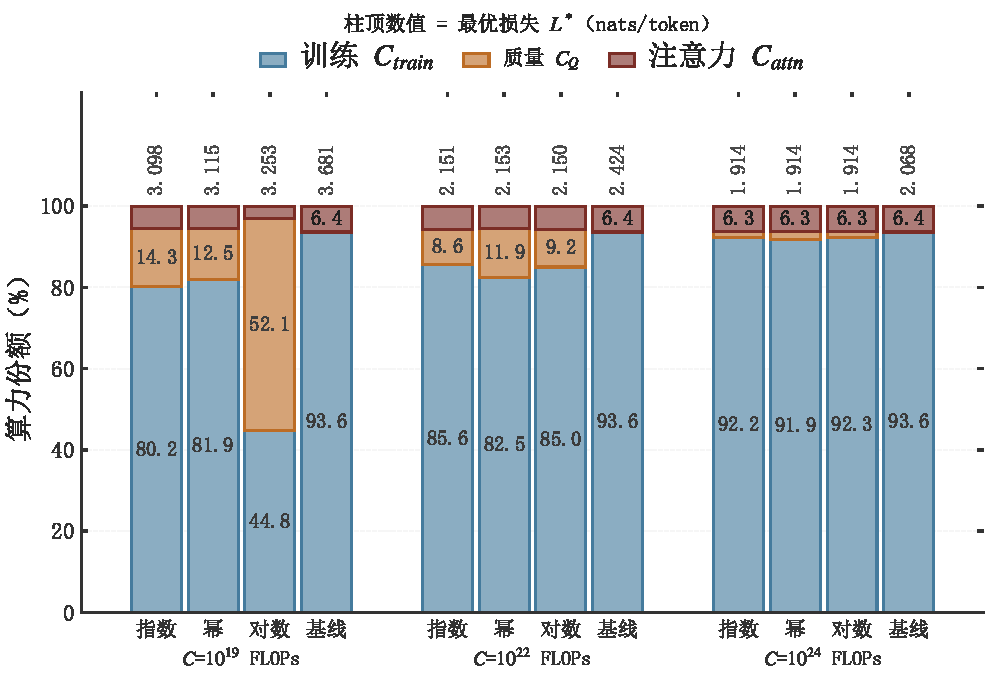
\includegraphics[width=0.9\textwidth,height=0.8\textheight,keepaspectratio]{fig_q3_allocation_stacked.pdf}
  \caption{三档预算下的算力份额构成}
  \label{fig:q3_allocation}
\end{figure}

基础训练份额始终主导（$0.80$--$0.92$），注意力份额随预算缓升，而质量提升份额在所示三档预算中随预算增大回落（图~\ref{fig:q3_allocation}）。这一份额变化提示资源结构可能转移，需要沿连续预算扫描定位。

\subsection{结构性转移的定义与识别}
给出可判定定义：以各部分算力份额 $s_X(C)=C_X^\ast/C$ 对预算对数的导数峰值定位转移点，
\begin{equation}
C^{\dagger}=\arg\max_{C}\ \left|\frac{\mathrm d\,s_X(C)}{\mathrm d\,\log C}\right| ,
\label{eq:q3-transition}
\end{equation}
并检查数值解是否触及质量边界或质量成本铰链。连续扫描预算对数区间、数值差分求份额导数可给出候选转移点；离散网格和成本函数选择会影响其位置。

\textbf{结果。}在当前 $\theta=0.5$、成本函数和扫描网格设定下，质量份额导数在预算约 $2.5\times10^{22}$ FLOPs 处出现峰值，作为模型内的候选结构转移点。基线质量 $0.079$ 较低，质量成本铰链在较低预算即已激活；这一结果同时依赖经验基线和假定的质量指数，不能称为纯数据驱动结论。转移点见图~\ref{fig:q3_transition}。

\begin{figure}[H]
  \centering
  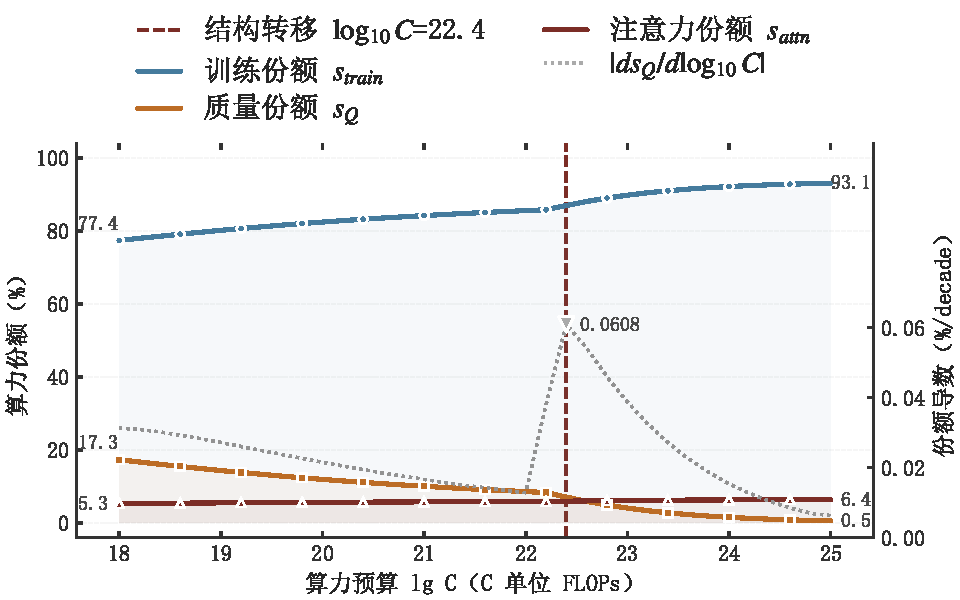
\includegraphics[width=0.9\textwidth,height=0.8\textheight,keepaspectratio]{fig_q3_transition_line.pdf}
  \caption{最优份额演化与结构性转移点}
  \label{fig:q3_transition}
\end{figure}

份额随预算对数演化曲线上叠加的份额导数，其峰值位置即由式~\eqref{eq:q3-transition} 定位的转移点（图~\ref{fig:q3_transition}）。由于该最优轨迹来自确定性优化、不存在重复抽样，图中不画置信带，而以份额导数曲线的峰值给出结构判据，当前实现未计算 KKT 残差，不能用一阶条件数值精度为转移位置背书。

\subsection{上下文长度的临界值与敏感性}
上下文长度为外生参数。令注意力开销等于训练开销 $\eta N\Dt\Lctx=6N\Dt$，与参数量、数据量无关，解得临界上下文
\begin{equation}
\Lctx^{\mathrm{crit}}=\frac{6}{\eta}=\frac{6}{2\times10^{-4}}=3\times10^{4}\ \text{tokens}.
\label{eq:q3-lctxcrit}
\end{equation}
当上下文长度达到该值时注意力开销与训练开销相当，超过它长上下文将显著挤压训练预算。敏感性扫描的取值严格取自模型架构元数据的实测集，即 $2048$、$4096$、$8192$、$32768$ 与 $131072$。图~\ref{fig:q3_lctx} 展示最优配置随上下文长度的变化。

\begin{figure}[H]
  \centering
  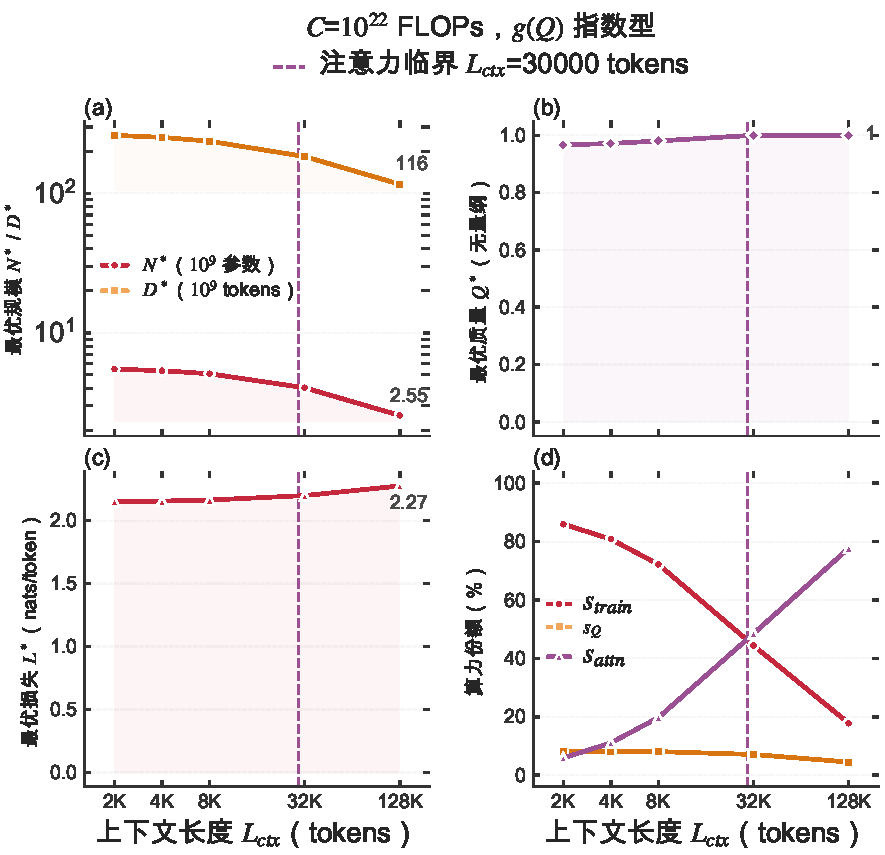
\includegraphics[width=0.92\textwidth,height=0.8\textheight,keepaspectratio]{fig_q3_lctx_panels.pdf}
  \caption{最优配置随上下文长度的变化}
  \label{fig:q3_lctx}
\end{figure}

在中档预算下，上下文由 $2048$ 增至 $131072$ 时，注意力份额从约 $0.058$ 升至约 $0.776$（图~\ref{fig:q3_lctx}）。临界值 $3\times10^{4}$ 位于 $8192$ 与 $32768$ 之间；上下文不小于 $32768$ 时，按当前成本模型，注意力开销超过基础训练开销，压缩了可用于参数量和数据量的预算。可行域见图~\ref{fig:tikz_q3_feasible}。

\begin{figure}[H]
  \centering
  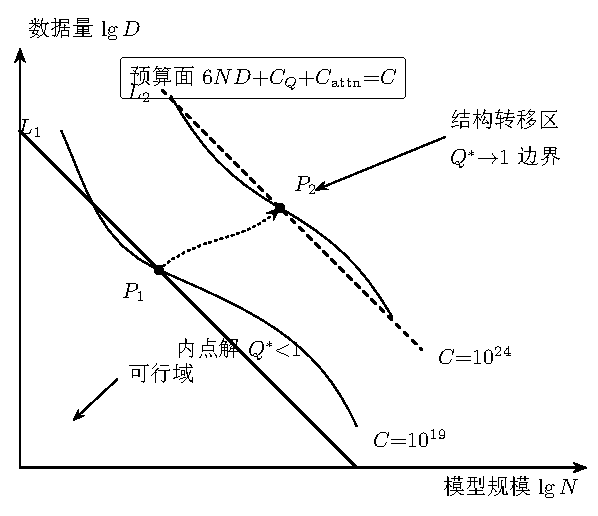
\includegraphics[width=0.8\textwidth,height=0.8\textheight,keepaspectratio]{tikz_q3_feasible.pdf}
  \caption{算力预算可行域与结构转移}
  \label{fig:tikz_q3_feasible}
\end{figure}

在参数量--数据量--质量空间中，由式~\eqref{eq:q3-budget} 界定的预算面、等成本线与最优点位置一同表明最优解落在预算面上（约束活跃），且随预算增大最优点沿预算面移动时穿过结构转移分区（图~\ref{fig:tikz_q3_feasible}）。综合本章：预算增大使损失单调改善并趋近不可约损失，最优策略在预算约 $2.5\times10^{22}$ 处发生质量投入结构的转移，长上下文以临界值 $3\times10^{4}$ 为界挤压训练预算。

\section{问题四：规模与非规模贡献分解、损失--基准桥接与能力前沿预测}

本章分析规模和年份与基准能力的关联，建立损失到基准的探索性桥接，最后在三档能力趋势假设下预测有许可证记录模型的经验前沿。

\subsection{综合能力度量与口径声明}
综合能力取六维基准均分（指令遵循、综合推理、数学、研究生级问答、多步推理与专业知识）：
\begin{equation}
\mathrm{Cap}=\frac{1}{6}\sum_{k=1}^{6} B_k,\qquad k\in\{\text{IFEval, BBH, MATH, GPQA, MUSR, MMLU-PRO}\}.
\label{eq:q4-cap}
\end{equation}
口径显式声明：前沿样本按榜单中许可证字段非空筛选；这只能视作“有许可证记录”的操作性代理，不能据此核实每个模型是否满足严格的开源定义\cite{llama2023,bloom2023}。时间轴用榜单年份，六维均分口径可复现。

\subsection{规模与年份项的描述性分解}
以榜单数据回归综合能力对规模变量与时间，检查两项在所选样本窗中的统计关联：
\begin{equation}
\mathrm{Cap}_i=f(\ln N_i)+h(t_i)+\varepsilon_i,
\label{eq:q4-decomp}
\end{equation}
其中规模项 $f$ 和时间项 $h$ 分别给出规模、年份与能力的统计关联。年份项可能同时吸收数据、训练配方、模型组成和评测变化，不能直接解释为纯技术进步。在时间窗 $[t_0,t_1]$ 上两项回归增量的形式占比为
\begin{equation}
\text{scale\%}=\frac{\Delta f}{\Delta f+\Delta h},\qquad
\text{nonscale\%}=\frac{\Delta h}{\Delta f+\Delta h},\qquad
\text{scale\%}+\text{nonscale\%}=100\% .
\label{eq:q4-share}
\end{equation}

\textbf{结果与识别假设。}在 $4561$ 个有效模型上回归得 $\mathrm{Cap}=-24576+6.27\ln N+12.14\,t$，决定系数 $0.462$；年份系数是控制参数量后的条件关联，不具因果解释。两变量之外仍有大量系统性变异。所选时间窗内平均参数规模下降，使回归规模项增量为负；按式~\eqref{eq:q4-share} 计算的两项份额约为 $-25\%$ 与 $125\%$。超出 $0$--$100\%$ 只是负增量下的比值结果，且分母由拟合增量而非观测到的能力变化构成。它只能描述这套回归与样本窗，不能据此证明非规模技术进步的因果份额。占比随时间的演化见图~\ref{fig:q4_contribution}。

\begin{figure}[H]
  \centering
  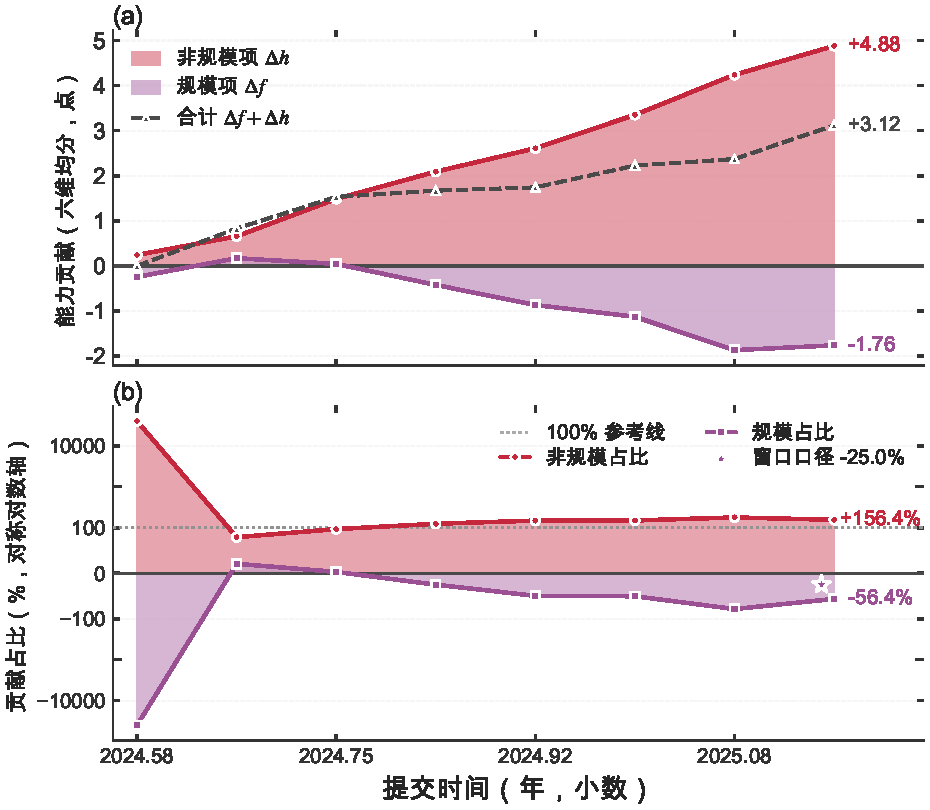
\includegraphics[width=0.92\textwidth,height=0.8\textheight,keepaspectratio]{fig_q4_contribution_decomp.pdf}
  \caption{规模与年份项的回归增量分解}
  \label{fig:q4_contribution}
\end{figure}

图~\ref{fig:q4_contribution} 用零线标明规模项在所选窗口内的负增量。该结果对时间窗、样本组成和回归设定敏感，适合作为描述性分解，不宜称规模为能力提升的净拖累。

\subsection{损失--基准桥接映射}
用同时含验证损失与六维基准的桥接样本建立损失到能力的单调映射，按可比性分层（高可比来自可与训练轨迹对照的模型，其余为中可比）。用单调递减的 sigmoid 型回归
\begin{equation}
\widehat{\mathrm{Cap}}=\frac{S_{\max}}{1+\exp\bigl(a(L-L_0)\bigr)}+c,\qquad a>0\ (\text{损失}\uparrow\Rightarrow\text{能力}\downarrow),
\label{eq:q4-bridge}
\end{equation}
分层拟合参数，并分别报告样本量与拟合误差。

\textbf{结果与不确定性。}高可比层样本仅 $7$ 条，决定系数约 $0.40$；中可比层 $68$ 条，决定系数约 $0.36$。映射只能作为损失到基准能力的探索性桥梁，不能给出可靠的模型外推精度。下一节的前沿直接由榜单能力值计算，不经过这条桥接，因此其预测区间不含桥接误差。图~\ref{fig:q4_bridge} 展示分层样本与拟合曲线。

\begin{figure}[H]
  \centering
  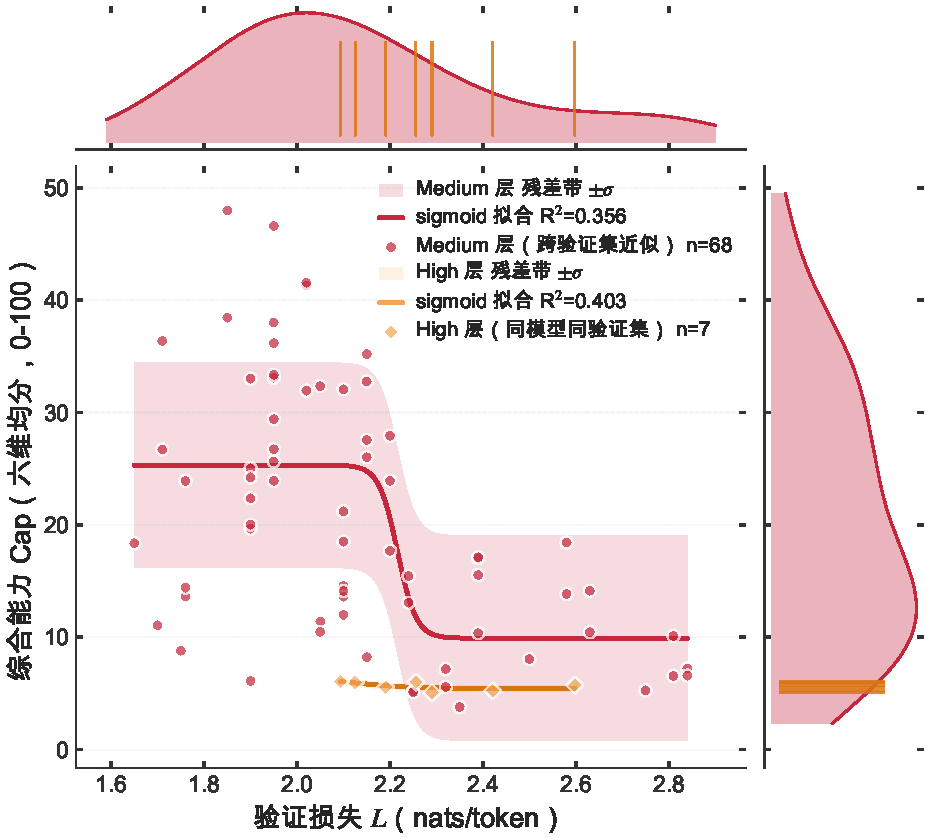
\includegraphics[width=0.92\textwidth,height=0.8\textheight,keepaspectratio]{fig_q4_bridge_scatter.pdf}
  \caption{损失到能力的分层桥接}
  \label{fig:q4_bridge}
\end{figure}

分层拟合的函数按约束随损失单调下降，但散点仍有较大离散（图~\ref{fig:q4_bridge}）。若用问题三的最优损失推算能力，必须另行传播桥接参数与残差的不确定性；此处未给出那类能力预测。

\subsection{能力趋势情景下的经验前沿预测}
将有许可证记录的模型按月分箱，至少有两条记录的月份取六维均分的第 $90$ 百分位作为经验前沿。实际有效月份仅 $10$ 个，覆盖约 $2024.46$ 至 $2025.21$。在这些月度点上拟合线性趋势；残差自助重采样后重新拟合斜率，并加入一次月度预测残差。以历史末值 $F_T$ 为锚，情景系数 $s\in\{0,0.5,1\}$ 缩放历史能力前沿斜率。第 $b$ 次自助样本在 $\Delta$ 个月后的预测为
\begin{equation}
F^{(b)}_{s,\Delta}=\operatorname{clip}_{[0,100]}
\left(F_T+s\,\hat\beta^{(b)}\frac{\Delta}{12}+\epsilon^{(b)}\right),
\qquad \Delta\in\{12,24\}.
\label{eq:q4-bootstrap}
\end{equation}
其中 $\hat\beta^{(b)}$ 是以重采样残差重新拟合的年斜率，$\epsilon^{(b)}$ 从同次残差样本抽取；共进行 $2000$ 次。对 $F^{(b)}_{s,\Delta}$ 取经验分位数，得到\emph{相对样本末点}约 $2026.21$ 和 $2027.21$ 的预测区间：
\begin{equation}
\mathrm{Frontier}(t+\Delta)\in\bigl[\hat F_{10}(t+\Delta),\ \hat F_{90}(t+\Delta)\bigr],\qquad \Delta\in\{12,24\}\ \text{月}.
\label{eq:q4-frontier}
\end{equation}
历史训练算力中位数约以每年 $5.1$ 倍增长，只为情景提供背景；数据并未估计训练算力增速与能力前沿斜率之间的弹性，因此三档系数是明确的假设。每个情景内的 $P_{10}$--$P_{90}$ 区间包含趋势估计和月度残差的不确定性；不同情景之间的差异须单独比较，桥接误差不参与计算。表~\ref{tab:q4_frontier} 汇总三情景结果。

\textbf{短期回测。}为检验线性趋势是否至少优于简单基线，从前 $5$ 个有效月度点开始，每次只用已观测点重新拟合并预测下一点，共得 $5$ 次一步预测。趋势模型的平均绝对误差为 $1.89$ 个能力点，平均误差（预测减实际）为 $+1.50$ 点；直接沿用上一月前沿的平均绝对误差为 $1.28$ 点。趋势模型在这一小样本回测中\emph{没有}优于末值延续，表明斜率外推存在乐观偏差风险。一步回测既不能校准 $12$--$24$ 个月区间，也无法覆盖未来模型组成变化；下表的远期数值仅作条件情景计算。

\begin{table}[H]
  \centering
  \caption{能力前沿情景预测分位数}
  \label{tab:q4_frontier}
  \small
  \begin{tabular}{llrrrr}
    \toprule
    情景 & 斜率系数 & 期限 & P10 & P50 & P90 \\
    \midrule
    维持 & 1.0 & 12 月 & 57.47 & 61.28 & 65.68 \\
     &  & 24 月 & 74.14 & 81.02 & 88.35 \\
    \addlinespace[2pt]
    放缓 & 0.5 & 12 月 & 48.97 & 51.38 & 54.90 \\
     &  & 24 月 & 57.47 & 61.28 & 65.68 \\
    \addlinespace[2pt]
    停滞 & 0.0 & 12 月 & 39.41 & 41.52 & 46.39 \\
     &  & 24 月 & 39.41 & 41.52 & 46.39 \\
    \addlinespace[2pt]
    \midrule
    历史末值 & -- & 2025.21 & \multicolumn{3}{r}{41.75} \\
    历史斜率 & -- & -- & \multicolumn{3}{r}{19.68 点/年} \\
    \bottomrule
  \end{tabular}
\end{table}


按上述假设，$24$ 个月中位数在系数 $1$、$0.5$、$0$ 下分别约为 $81$、$61$、$42$（表~\ref{tab:q4_frontier}）。零斜率情景的 $12$ 与 $24$ 个月分布相同；其余情景随时间上升是线性趋势和正系数的模型结果，不是已验证的能力不倒退规律。历史末值约 $42$、拟合斜率约 $20$ 点每年；以不足一年数据外推两年，绝对数值应谨慎使用。前沿分位带见图~\ref{fig:q4_frontier}。

\begin{figure}[H]
  \centering
  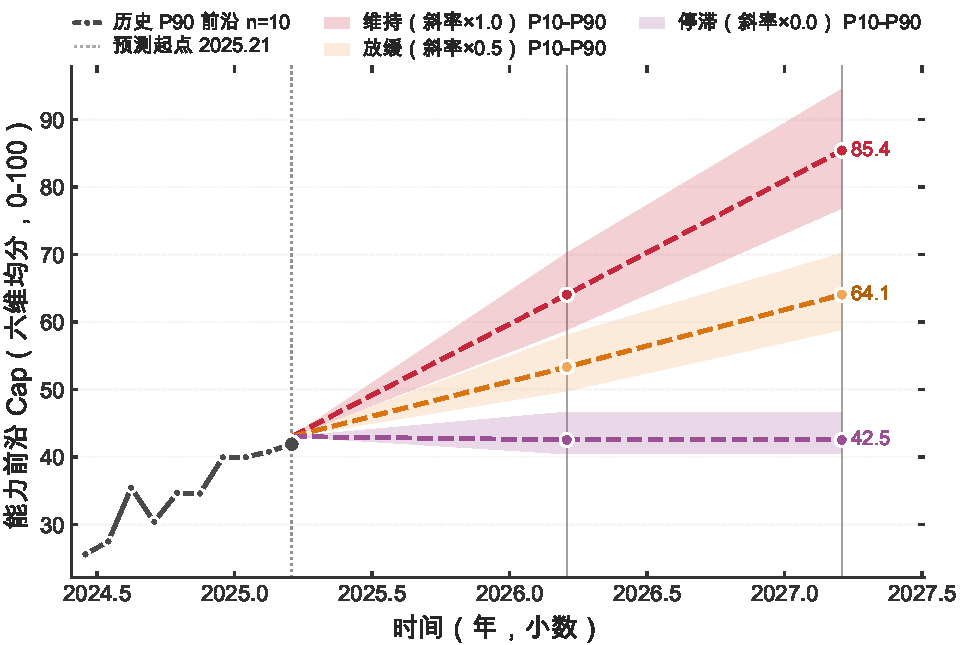
\includegraphics[width=0.9\textwidth,height=0.8\textheight,keepaspectratio]{fig_q4_frontier_fan.pdf}
  \caption{能力前沿情景预测区间}
  \label{fig:q4_frontier}
\end{figure}

图~\ref{fig:q4_frontier} 展示各情景内的 $10\%$--$90\%$ 分位带；零斜率情景的区间不随期限扩大，另两档随斜率估计误差扩大。图中超出历史范围的部分均为情景外推，纵轴为六维基准均分 $0$--$100$。有限月度点、样本组成变化和情景映射假设均未被区间充分覆盖。

\subsection{逐任务聚合分析}
仅用榜单汇总列不足以刻画能力短板，本文遍历逐任务评测记录，按目录取最新可解析记录、跳过损坏文件做逐任务聚合。共解析 $1860$ 个目录（六维完整 $1854$、损坏跳过 $7$），覆盖满足要求。各任务难度均值为：指令遵循 $40.2$、综合推理 $47.5$、数学 $11.4$、研究生级问答 $29.8$、多步推理 $40.0$、专业知识 $32.0$，其中数学最难。图~\ref{fig:q4_task_radar} 展示前沿模型的六维剖面。

\begin{figure}[H]
  \centering
  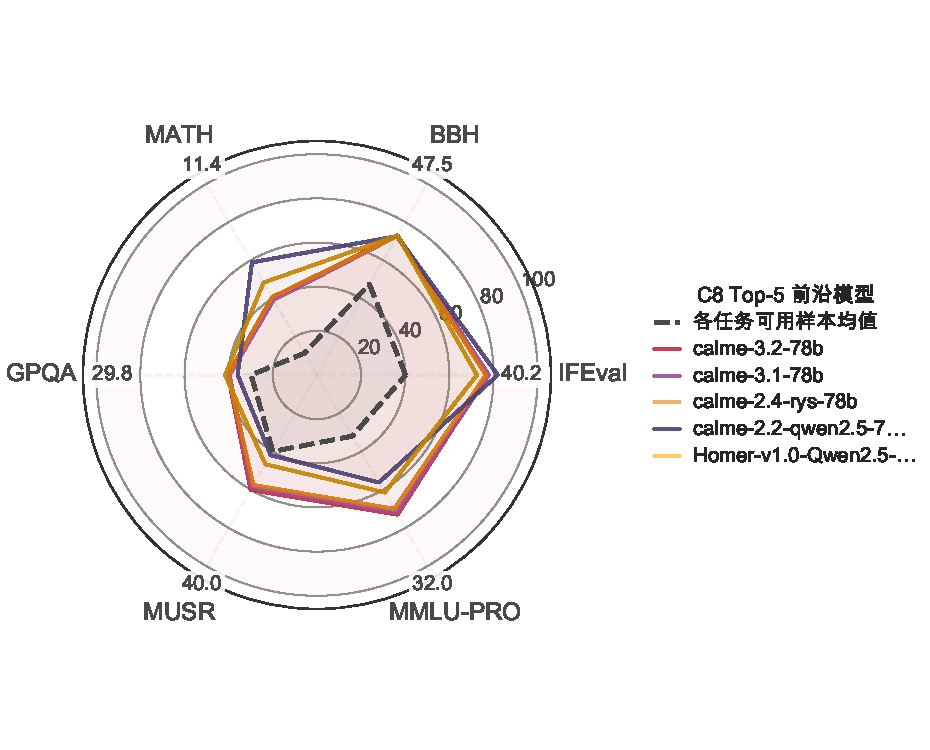
\includegraphics[width=0.92\textwidth,height=0.8\textheight,keepaspectratio]{fig_q4_task_radar.pdf}
  \caption{前沿模型逐任务能力剖面}
  \label{fig:q4_task_radar}
\end{figure}

前沿模型在综合推理与指令遵循维度较强，而在数学与研究生级问答维度普遍偏弱，六维剖面的不均衡揭示了当前能力短板集中在高难推理任务上（图~\ref{fig:q4_task_radar}）\cite{mmlu2020}。这与式~\eqref{eq:q4-cap} 均分口径下的综合能力互为补充：均分给出总体水平，逐任务剖面给出结构短板。

% 仅此处允许问题四末图跨到下一节页顶，让模型检验正文回填上一页余白。
\begingroup
\let\FloatBarrier\relax
\section{模型检验与灵敏度分析}

本章对四个模型的关键结论作独立复核，并对高敏感假设做扰动分析，说明结果的适用范围。

\subsection{独立复核}
问题一另以不导入主评分模块的脚本从压缩原始记录重算，$51230$ 条 A1 逐条分数与保存值最大差异为 $2.3\times10^{-16}$，A2/A3 的域均值与冲突计数均一致。与 CRITIC、$22$ 项等权、argmax 解码的七域排序 Kendall 相关分别为 $0.333$、$0.238$、$0.810$，提示权重选择是主要不确定来源；A2/A3 的同名域均值接近 A1，不能证明其余域的泛化性。问题二的经典律在四组独立数据上分层验证；广义律在留出集的均方根误差 $0.688$ 低于同参经典基线 $0.971$，但 $Q=1$ 的零退化误差是公式恒等式。问题三把候选配置重代入物理 FLOPs 公式核验，三项总算力均未超预算；多起点与预算回代不能证明全局最优。问题四的一步滚动回测中，趋势模型平均绝对误差 $1.89$ 高于末值延续的 $1.28$。

\subsection{灵敏度分析}
质量放大指数 $\theta$ 不是可由现有质量标度识别的估计量，故对 $Q_0$ 与 $\theta$ 分别作条件扰动。在指数型质量成本、$\Lctx=2048$ 和同一多起点求解规则下，重求三档预算的候选配置；结果见表~\ref{tab:q3-assumption-sensitivity}。

\begin{table}[H]
  \centering
  \caption{质量基线与指数扰动下的候选最优质量}
  \label{tab:q3-assumption-sensitivity}
  \small
  \begin{tabular}{lrrrrr}
    \toprule
    情景 & $Q_0$ & $\theta$ & $Q^\ast_{10^{19}}$ & $Q^\ast_{10^{22}}$ & $Q^\ast_{10^{24}}$ \\
    \midrule
    基准 & 0.0789 & 0.5 & 0.546 & 0.968 & 1.000 \\
    $Q_0$ 降 20\% & 0.0631 & 0.5 & 0.546 & 0.968 & 1.000 \\
    $Q_0$ 升 20\% & 0.0947 & 0.5 & 0.545 & 0.968 & 1.000 \\
    $\theta=0.2$ & 0.0789 & 0.2 & 0.417 & 0.823 & 1.000 \\
    $\theta=0.8$ & 0.0789 & 0.8 & 0.623 & 1.000 & 1.000 \\
    \bottomrule
  \end{tabular}
\end{table}


$Q_0$ 上下扰动 $20\%$ 时，低预算候选质量从基准 $0.506$ 变为 $0.528$ 或 $0.585$；中预算约 $0.965$--$0.967$，高预算均为 $1$。因此低预算结果对新基线并非不敏感。固定 $Q_0$ 而将 $\theta$ 从 $0.2$ 改为 $0.8$，低预算质量由 $0.488$ 升至 $0.585$，中预算由 $0.821$ 升至边界 $1$。不同 $\theta$ 对应不同损失函数，情景间损失值不能解释为模型性能提升。

冲突降权因子 $\delta\in\{0.3,0.5,0.7,1.0\}$ 的扫描中七域排序均不变。三型质量成本在低预算的候选 $Q$ 为 $0.506$、$0.488$、$0.488$；中预算差异更大，为 $0.967$、$1$、$1$。能力前沿的三档斜率系数决定情景间差异，每档内的自助区间只覆盖趋势估计和月度残差，不包含情景选择或结构性模型误差。

\subsection{适用范围}
经典律的直接拟合支撑范围约为参数量 $0.07$--$12$、数据量至 $300$（均以 $10^9$ 计）；问题三的高预算解已超出该范围，其损失是公式外推。质量指数与能力前沿斜率系数均为高敏感假设，替代率、转移点及远期能力水平不宜作确定性解读。前沿仅有 $10$ 个有效月度点，短期回测也未证明趋势模型优于简单基线。

\endgroup
\section{模型评价、改进与推广}

\subsection{模型优点}
本文四问覆盖从数据刻画到能力预测的主要环节，但数值链条仍有断点：问题一的域级质量用于问题三的质量成本基线；配比贡献尚未进入广义律数值计算；损失到能力的桥接是单独拟合的探索性映射。A1 固定参照与逐条复核使质量评分可重算；广义律在 $Q=1$ 时满足代数退化。优化部分用 KKT 刻画结构、预算消元与质量剖面搜索候选解，并以份额导数峰值定义候选结构转移。对半合成质量标度方向异常和前沿窗口规模负增量均保留并讨论。

\subsection{模型不足与改进方向}
其一，质量放大指数无法从唯一一组半合成数据识别，其经验拟合落在边界且口径与部署质量不同，故下游采用了反映“质量有益”前提的取值并做敏感性；若能获得大规模真实的质量--损失联合观测，可把该指数从假设升级为估计。其二，配比没有进入当前标度律数值计算，也未联立优化 $17$ 维配比；改进可把配比加入决策变量并以投影梯度处理单纯形约束，代价是转移分析的可解释性下降。其三，前沿预测依赖能力斜率情景假设，并未估计算力增速到能力斜率的映射，改进可引入更细的算力供给模型或以真实新发布模型滚动校正分位带。

\subsection{推广}
广义标度律的“有效数据量”形式可推广到其它可归一化的数据属性（如去重率、领域纯度），并在归一化边界 $Q=1$ 退化为经典形式。问题三的三部分算力约束可扩展到含推理成本或多阶段训练的预算结构。问题四的描述性分解与分层桥接可用于其它基准体系；这些推广均需在目标场景重新标定参数。

\section{结论}
本文用语义解码、A1 固定百分位参照和三组平衡权重重算问题一，得七域质量中位数 $Q_0=0.48788$；按高教育价值且判有广告的规则，A1 冲突率为 $0.303\%$，其中 C4 的域内冲突率最高，为 $1.03\%$。配比模型在同尺度检验上具有一定解释力，但跨尺度绝对损失预测失准。经典标度律拟合良好；广义律的质量指数仍属结构性假设。在新 $Q_0$ 下，指数型质量成本的三档预算候选最低损失为 $3.073$、$2.151$、$1.914$，质量份额变化峰值约在 $10^{19}$ FLOPs；注意力与基础训练开销相当的上下文长度为 $3\times10^{4}$ tokens。能力前沿预测依赖情景斜率，不能视为已校准的无条件预测。质量分数与资源配置结论的主要限制是评分权重及成本函数尚无训练损失标签的联合校准。


% 参考文献与附录顺排，避免强制分页在章节尾部留下大片空白。
\FloatBarrier
\clearpage
\begin{thebibliography}{99}
\small

\bibitem{metarater}
OpenDataLab. SlimPajama-Meta-rater dataset card, field descriptions.
\url{https://huggingface.co/datasets/opendatalab/SlimPajama-Meta-rater}.

\bibitem{kaplan2020}
Kaplan J, McCandlish S, Henighan T, et al.
Scaling Laws for Neural Language Models.
arXiv:2001.08361, 2020. DOI: 10.48550/arXiv.2001.08361.

\bibitem{hoffmann2022}
Hoffmann J, Borgeaud S, Mensch A, et al.
Training Compute-Optimal Large Language Models.
arXiv:2203.15556, 2022. DOI: 10.48550/arXiv.2203.15556.

\bibitem{regmix2024}
Liu Q, Zheng X, Muennighoff N, et al.
RegMix: Data Mixture as Regression for Language Model Pre-training.
arXiv:2407.01492, 2024. DOI: 10.48550/arXiv.2407.01492.

\bibitem{doremi2023}
Xie S M, Pham H, Dong X, et al.
DoReMi: Optimizing Data Mixtures Speeds Up Language Model Pretraining.
arXiv:2305.10429, 2023. DOI: 10.48550/arXiv.2305.10429.

\bibitem{fineweb2024}
Penedo G, Kydl\'i\v{c}ek H, Ben Allal L, et al.
The FineWeb Datasets: Decanting the Web for the Finest Text Data at Scale.
arXiv:2406.17557, 2024. DOI: 10.48550/arXiv.2406.17557.

\bibitem{slimpajama2023}
Shen Z, Tao T, Ma L, et al.
SlimPajama-DC: Understanding Data Combinations for LLM Training.
arXiv:2309.10818, 2023. DOI: 10.48550/arXiv.2309.10818.

\bibitem{dsir2023}
Xie S M, Santurkar S, Ma T, Liang P.
Data Selection for Language Models via Importance Resampling.
arXiv:2302.03169, 2023. DOI: 10.48550/arXiv.2302.03169.

\bibitem{qurating2024}
Wettig A, Gupta A, Malik S, Chen D.
QuRating: Selecting High-Quality Data for Training Language Models.
arXiv:2402.09739, 2024. DOI: 10.48550/arXiv.2402.09739.

\bibitem{pile2020}
Gao L, Biderman S, Black S, et al.
The Pile: An 800GB Dataset of Diverse Text for Language Modeling.
arXiv:2101.00027, 2020. DOI: 10.48550/arXiv.2101.00027.

\bibitem{pythia2023}
Biderman S, Schoelkopf H, Anthony Q, et al.
Pythia: A Suite for Analyzing Large Language Models Across Training and Scaling.
arXiv:2304.01373, 2023. DOI: 10.48550/arXiv.2304.01373.

\bibitem{gpt3_2020}
Brown T B, Mann B, Ryder N, et al.
Language Models are Few-Shot Learners.
arXiv:2005.14165, 2020. DOI: 10.48550/arXiv.2005.14165.

\bibitem{emergent2022}
Wei J, Tay Y, Bommasani R, et al.
Emergent Abilities of Large Language Models.
arXiv:2206.07682, 2022. DOI: 10.48550/arXiv.2206.07682.

\bibitem{mirage2023}
Schaeffer R, Miranda B, Koyejo S.
Are Emergent Abilities of Large Language Models a Mirage?
arXiv:2304.15004, 2023. DOI: 10.48550/arXiv.2304.15004.

\bibitem{helm2022}
Liang P, Bommasani R, Lee T, et al.
Holistic Evaluation of Language Models.
arXiv:2211.09110, 2022. DOI: 10.48550/arXiv.2211.09110.

\bibitem{mmlu2020}
Hendrycks D, Burns C, Basart S, et al.
Measuring Massive Multitask Language Understanding.
arXiv:2009.03300, 2020. DOI: 10.48550/arXiv.2009.03300.

\bibitem{llama2023}
Touvron H, Lavril T, Izacard G, et al.
LLaMA: Open and Efficient Foundation Language Models.
arXiv:2302.13971, 2023. DOI: 10.48550/arXiv.2302.13971.

\bibitem{bloom2023}
Le Scao T, Fan A, Akiki C, et al.
BLOOM: A 176B-Parameter Open-Access Multilingual Language Model.
arXiv:2211.05100, 2023. DOI: 10.48550/arXiv.2211.05100.

\bibitem{quantile2001}
Koenker R, Hallock K F.
Quantile Regression.
Journal of Economic Perspectives, 2001, 15(4): 143--156. DOI: 10.1257/jep.15.4.143.

\bibitem{sqp1995}
Boggs P T, Tolle J W.
Sequential Quadratic Programming.
Acta Numerica, 1995, 4: 1--51. DOI: 10.1017/S0962492900002518.

\bibitem{entropy_topsis}
Chen C H.
A Novel Multi-Criteria Decision-Making Model for Building Material Supplier Selection Based on Entropy-AHP Weighted TOPSIS.
Entropy, 2020, 22(2): 259. DOI: 10.3390/e22020259.

\end{thebibliography}

% DATA_CHECK_PASSED

\clearpage
\appendix
\section{附录：参数取值与求解步骤}

\subsection{题面给定常量与成本函数}
问题三的算力构成与质量成本参数按题面原样载入，列于表~\ref{tab:appendix-params}。

\begin{table}[!htbp]
  \centering
  \songti\zihao{-4}
  \caption{题面给定常量与三型质量成本参数}
  \label{tab:appendix-params}
  \begin{tabular}{lll}
    \toprule
    物理量 & 取值 & 说明 \\
    \midrule
    注意力系数 $\eta$ & $2\times10^{-4}$ & 作用于三者乘积 $N\Dt\Lctx$ \\
    Chinchilla 系数 & $6$ & 每参数每 token 的训练算力 \\
    注意力临界上下文 & $3\times10^{4}$ & 由 $6/\eta$ 解析得到 \\
    指数型 $g(Q)$ & $10^{7}\,e^{6Q}$ & 高质量极昂贵 \\
    幂型 $g(Q)$ & $5\times10^{9}\,Q^{4}$ & 高质量成本居中 \\
    对数型 $g(Q)$ & $2\times10^{9}\ln(1+10Q)$ & 高质量相对可得 \\
    三档预算 $C$ & $10^{19},10^{22},10^{24}$ & FLOPs \\
    基线质量 $Q_0$ & $0.48788$ & 问题一七域质量中位数 \\
    \bottomrule
  \end{tabular}
\end{table}

三型质量成本函数在中高预算下给出相近的最优质量，但在低预算档因高质量的经济性不同而分化，这是问题三比较成本函数选择影响的依据（表~\ref{tab:appendix-params}）。

\subsection{优化求解步骤}
问题三先利用预算活跃条件消去 $D$，在每个固定质量下求唯一的 $\ln N$ 驻点，再以质量网格、局部细化和端点比较选取候选。所有结果复算预算以及质量单边条件；另用 $513$ 点加密网格及 $20$ 起点 SLSQP 核验九组主预算。连续预算扫描输出份额导数和质量边界阈值。求解器一致性与局部残差不构成全局最优证明。

\subsection{关于人工智能工具的使用说明}
本文使用通用大语言模型辅助代码检查与修改、公式推导核验、图表生成、文字润色及 LaTeX 排版。报告数值以随文程序对题目附件的计算及已声明公式的复算为依据；模型假设、经验观测和情景外推分别标明，工具输出通过对应的数值检查后写入正文。

\section{附录：核心算法代码摘录}
\label{app:core-code}

下列代码摘自随文提交的计算脚本，仅展示关键算法；数据摄入、绘图和结果写出等实现不在纸质附录展开。完整程序见电子材料的 \texttt{code/}，问题一的语义解码和固定参照评分见 \texttt{quality\_scoring.py} 与 \texttt{q1\_pipeline.py}。

% 以下 firstline/lastline 对应随文提交的源文件；修改源文件时须同步核对范围。

\subsection{问题一：质量评分与配比回归}

\lstinputlisting[style=pythonstyle,firstline=41,lastline=75,caption={二分类与六分类信号的语义解码},label={code:q1-score}]{../code/quality_scoring.py}

\lstinputlisting[style=pythonstyle,firstline=117,lastline=142,caption={A1 固定百分位与三组平衡评分},label={code:q1-quality}]{../code/quality_scoring.py}

\lstinputlisting[style=pythonstyle,firstline=54,lastline=59,caption={高教育价值与广告判定的冲突条件},label={code:q1-conflict}]{../code/q1_pipeline.py}

\lstinputlisting[style=pythonstyle,firstline=55,lastline=72,caption={单纯形配比回归及可识别系数编码},label={code:q1-mixture}]{../code/problem1.py}

\subsection{问题二：经典与广义标度律}

\lstinputlisting[style=pythonstyle,firstline=37,lastline=67,caption={经典标度律的对数域稳健拟合},label={code:q2-classic}]{../code/problem2.py}

\lstinputlisting[style=pythonstyle,firstline=70,lastline=117,caption={广义标度律及质量指数拟合},label={code:q2-generalized}]{../code/problem2.py}

\subsection{问题三：预算约束下的资源配置}

\lstinputlisting[style=pythonstyle,firstline=114,lastline=169,caption={预算消元、质量剖面搜索与边界检验},label={code:q3-solver}]{../code/problem3.py}

\subsection{问题四：能力前沿与情景预测}

\lstinputlisting[style=pythonstyle,firstline=190,lastline=211,caption={单调有界的损失到能力桥接},label={code:q4-frontier}]{../code/problem4.py}

\lstinputlisting[style=pythonstyle,firstline=325,lastline=351,caption={联合重拟合截距与斜率的自助情景预测},label={code:q4-forecast}]{../code/problem4.py}


\end{document}
